\documentclass[11pt,english,a4paper]{article}
\usepackage{natbib, amsmath, amsfonts, units, graphicx, hyperref, txfonts, fleqn, geometry, pifont, setspace, eurosym, afterpage, caption, subcaption, array, booktabs, ragged2e}
\usepackage{fancyhdr}

% Override daft defaults for float positioning
\renewcommand{\topfraction}{0.9}	% max fraction of floats at top
\renewcommand{\bottomfraction}{0.8}	% max fraction of floats at bottom
% -- Text pages
\setcounter{topnumber}{2}
\setcounter{bottomnumber}{2}
\renewcommand{\textfraction}{0.07}
% -- Float pages
\renewcommand{\floatpagefraction}{0.7}

\providecommand{\keywords}[1]{\textbf{\textit{Keywords ---}} #1}
\renewcommand*{\bibfont}{\small}
\setlength{\bibsep}{0.0pt}

\captionsetup[figure]{labelfont={small,bf},textfont=small,justification=raggedright,labelsep=space,singlelinecheck=false}
\captionsetup[table]{labelfont={small,bf},textfont=small,justification=raggedright,labelsep=space,singlelinecheck=false}

\pagestyle{fancy}
\fancyhf{}
\lhead{Liang Q and Smith LS (2015)}
\rhead{}
\cfoot{\thepage}

\title{A High-Performance Integrated Hydrodynamic Modelling System for Urban Flood Simulations}
\author{Qiuhua Liang,\\
	State Key Laboratorty of Hydrology, Water \\
	Resources and Hydraulic Engineering,\\
	Hohai University \\
	\texttt{qiuhua.liang@ncl.ac.uk}
	\thanks{Telephone: +44 (0) 191 208 6413}
	\and
	Luke S. Smith,\\
	School of Civil Engineering \\
	and Geosciences,\\
	Newcastle University\\
	\texttt{l.s.smith@ncl.ac.uk}
}
\date{\vspace*{12.0pt}Accepted \textbf{18 December 2014} \\ Published online \textbf{20 January 2015}}

\begin{document}
\maketitle

\begin{abstract}
A new High-Performance Integrated hydrodynamic Modelling System (Hi-PIMS) is tested for urban flood simulation. The software solves the two-dimensional shallow water equations (SWEs) using a first-order accurate Godunov-type shock-capturing scheme incorporated with the Harten, Lax and van Leer approximate Riemann solver with the contact wave restored (HLLC) for flux evaluation. The benefits of modern graphics processing units (GPUs) are explored to accelerate large-scale high-resolution simulations. In order to test its performance, the tool is applied to predict flood inundation due to rainfall and a point source surface flow in Glasgow, Scotland, and a hypothetical inundation event at different spatial resolutions in Thamesmead, England caused by embankment failure. Numerical experiments demonstrate potential benefits for high-resolution modelling of urban flood inundation, and a much-improved level of performance without compromising result quality.
\end{abstract}
\keywords{urban flood inundation, hydrodynamic model, finite-volume Godunov-type scheme, shallow water equations, graphics processing unit, Hi-PIMS}

\vfill
\noindent\fbox{
\begin{minipage}{\dimexpr\textwidth-2\fboxsep-2\fboxrule}
\small
This is the authors' version of a work that was accepted for publication in the Journal of Hydroinformatics. A definitive version was subsequently published in the Journal of Hydroinformatics online. doi:\url{http://dx.doi.org/10.2166/hydro.2015.029}
\end{minipage}
}

\section{Introduction}

The past year of 2012 has seen the UK and numerous regions around the world subjected to an unusually wet summer, causing severe flash flooding. In July, August and September, many places in the UK, including Wales, Cornwall, Devon, North Somerset, North and West Yorkshire, Newcastle and the Scottish Borders, suffered flash flooding that caused substantial damage to property and major disruption to transport networks. Outside of the UK, a devastating flood killed 144 people in the Krasnodar region of Russia in July; Beijing in China, Uttarakhard in India and Manilla in the Phillipines have also been struck since. Most commonly associated with torrential rainfall, these flash floods are characterised by a sudden rise in river and subsequent floodplain inundation, and high-velocity overland flow following a rapid catchment response to the intense rainfall. Numerous processes related to the catchment response including bore formation (so-called 'walls of water') remain poorly understood but numerical modelling provides a means through which these events may be reproduced. Reliable simulation of these violent and unpredictable natural events demands a shock-capturing hydrodynamic model, generally beyond the capabilities of hydrological and simplified hydraulic modelling. However, the high computational burden associated with full hydrodynamic models has restricted their wider application to small spatial extents and short duration events. Most of the existing shock-capturing hydrodynamic models are not able to provide efficient and high-resolution simulations for large-scale flash flood events. Particularly, most of the aforementioned flash floods occur in urban areas, where high-resolution simulation is essential in order to resolve the complex urban topographic features consisting of buildings, streets and embankments in order to provide reliable numerical predictions. This poses a great challenge to existing two-dimensional hydrodynamic flood modelling tools, which are generally computationally demanding. This work therefore presents a new High-Performance Integrated hydrodynamic Modelling System (Hi-PIMS) for efficient high-resolution urban flood modelling.

Considerable research effort has been directed towards acceleration of flood modelling in order to achieve higher spatial resolutions and greater extents. Much of this literature focusses on simplification of the underlying equations to create kinematic- or diffusive-wave approximations. However, most of these simplified models are not appropriate to depict the complex catchment responses hypothesised whilst providing accurate depths and velocities, and their reduced physical complexity may cause increased sensitivity to and dependence on parameterisation \citep{Costabile2009,Costabile2012,Fewtrell2011a,Yeh2011}. Furthermore, there is evidence to suggest these simplified approaches will not achieve significant and consistent reductions in computation time, albeit case and resolution dependent \citep{Hunter2007,Pender2010,Wang2011a}. In order to improve computational efficiency of the diffusion-wave models for high-resolution simulations, \citet{Bates2010} presented a new formula for estimating inter-cell discharges for this type of models by partially restoring the inertial terms from the fully dynamic momentum equation. The numerical stability of the resulting partial inertial model is now controlled by the much less restricted Courant\textendash Freidrichs\textendash Lewy (CFL) condition, identical to the explicit hydrodynamic models. Due to the use of simplified governing equations and a simpler numerical scheme, the partial inertial model is shown to save 20\% - 30\% of the computational cost by comparison with a shock-capturing hydrodynamic model that solves the full two-dimensional shallow water equations in the similar code base \citep{Zhang2014}. However, for a city-scale high-resolution flood simulation that covers millions of computational nodes, the partial inertial models are still computationally too demanding. Furthermore, \citet{Neal2012}, after comparing the performance of their diffusion-wave, partial inertial and shock-capturing dynamic wave models against a set of benchmark test cases, pointed out that while the simplified models may reproduce numerical results comparable to a full model they are unable to simulate supercritical flows accurately. However, urban flash flood events as a result of intense rainfall or failure of flood defences are generally characterised as rapidly varying trans-critical and supercritical flows. Therefore, the shock-capturing fully dynamic models, representing the most recent developments in simulating complex shallow flow hydrodynamics, appear to be a natural option for urban flash flood modelling as considered in this work, although they are still inadequate in representing certain small-scale three-dimensional flow features \citep{Soares-Frazao2008,Guinot2012}. 

By creating a refined mesh only in those areas of interests, dynamic grid adaption provides an effective means to relax the high computational burden inherent in the full dynamic inundation models. While retaining the robustness and complexity of the numerical approach, dynamic grid adaptation however presents new problems if mass conservation is to be achieved. It is unlikely to increase the timestep for cases where the highest level of refinement is concentrated on the most complex flow dynamics and highest velocities or free-surface gradients \citep[see descriptions of refinement criteria in][]{Liang2008a,Kubatko2009}.

Rather than creating high-resolution mesh to directly capture small-scale topographic or flow features as used in the adaptive mesh methods, different sub-grid parameterization techniques have also been proposed to integrate high-resolution topographic features into flood models to enable more accurate and efficient coarse-resolution simulations \citep[e.g.][]{Soares-Frazao2008,Guinot2012,Schubert2012,Chen2012}. Most of these models are essentially based on rigorous reformulation of full dynamic shallow water equations to effectively reproduce complex urban topography \citep[e.g.][]{Soares-Frazao2008,Guinot2012,Schubert2012}. \citet{Soares-Frazao2008} introduced a new shallow flow model with porosity to account for the reduction in storage due to sub-grid topographic features. The performance of the porosity model was compared with that of a refined mesh model explicitly reflecting sub-grid scale urban structures and a more classical approach of raising local bed roughness. While able to reproduce the mean characteristics of the urban flood waves at a much lower computational cost than the refined mesh simulations, the porosity model was unable to accurately predict the formulation and propagation of certain localised wave features, e.g. reflected bores. In another study, \citet{Schubert2012} investigated various approaches of representing sub-grid topographic features in simulating a dam-break flood in an urban area and concluded that only those methods taking into account of building geometries can capture building-scale variability in the velocity field. They also indicated the benefit of using high-resolution simulation to explicitly represent buildings and road structures if run-time execution costs were not a major concern \citep[see also][]{Gallegos2009}. The issue of high-computational cost may be resolved by exploring recent developments in computational hardware.

If software developers are to keep pace with the increasing power of hardware, they must accept and respond to the stagnation of Central Processing Unit (CPU) clock speeds and look to parallel processing to fully harness computing power. Despite this the majority of commercial hydraulic modelling software can only utilise a single CPU core. Parallel programming approaches are shown to exhibit good weak and strong scaling when software is structured appropriately \citep[e.g.][]{Neal2010,Saetra2012}. But there is a far more interesting potential for looking beyond the CPU and examining the role heterogeneous computing might play. Graphics Processing Units (GPUs) are designed to process large volumes of data by performing the same calculation numerous times, typically on vectors and matrices. Such hardware architectures are well-suited to the field of computational fluid dynamics. New programming languages including CUDA and OpenCL have exposed this hardware for use in general-purpose applications (GPGPU). A number of attempts have been made to explore the benefits of GPU computing for highly efficient large-scale flood simulations. Early pioneers of such methods include \citet{Crossley2009} who harnessed graphics APIs directly to implement a diffusion wave model (JFlow) for GPUs, \citet{Kalyanapu2011} with a finite-difference implementation of the full shallow water equations, and later \citet{Brodtkorb2012} with a finite-volume scheme. Such software is becoming increasingly mainstream; \citet{Pender2013} report results from several commercial GPU hydraulics implementations while \citet{Smith2013} demonstrate the potential for generalised approaches applicable to both CPU and GPU co-processors. The most recent research also explores how domain decomposition across multiple GPUs can provide further performance benefits \citep{Saetra2012}. 

This work aims to present a high-performance hydrodynamic model for simulating different types of urban inundation processes including those induced flash floods, which generally involves rapidly-varying transcritical flows that should be reliably resolved by a robust shock-capturing shallow water model. The new computational power provided by recent developments in GPU computing is explored by adopting the model framework as introduced in \citet{Smith2013}, which solves the 2D shallow water equations using a 2nd-order accurate shock-capturing finite-volume Godunov-type scheme. The model can take advantage of either CPUs or GPUs with a single codebase by leveraging OpenCL. To further improve the computational efficiency of the modelling framework, a 1st-order accurate scheme is implemented, due to the fact that a 2nd-order accurate numerical scheme may not always be superior in real-world applications \citep{Zhang2013}. Extra source and sink terms are also included in the new implementation to better describe the urban rainfall-runoff processes. With Hi-PIMS, the focus of this work is to demonstrate that high-resolution large-scale urban inundation modelling can be realised at an affordable computational cost. Application to a standard benchmark test in Glasgow and a hypothetical case at Thamesmead reaffirms its efficiency and suitability. Results are presented for different vendors' devices.

\section{Finite-volume Godunov-type shallow flow solver}

In the general case for a flood event, the water depth is much smaller than the horizontal dimensions of the water body. Therefore the hydrodynamics of the flood wave can be suitably described by the shallow water equations (SWEs) that are derived to take full account of mass and momentum conservation in a two-dimensional manner. In matrix form, the SWEs may be written as

\begin{equation}
	\label{SWE_1stO}
	\frac{\partial\textbf{u}}{\partial t} +
	\frac{\partial\textbf{f}}{\partial x} +
	\frac{\partial\textbf{g}}{\partial y} =
	\textbf{s} ,
\end{equation}

where $t$ is the time, $x$ and $y$ the Cartesian coordinates, $q$ the vector representing the flow variables, $f$ and $g$ the fluxes in the two Cartesian directions, and $s$ is the source term vector. The vector terms are given by \citet{Liang2009b},

\renewcommand{\arraystretch}{1.5}
\begin{equation}
	\label{SWETerms_1stO}
	\begin{alignedat}{4}
		&\textbf q && = \left[ \begin{array}{c}
			\eta \\
			q_x \\
			q_y
		\end{array} \right] , \hspace{4ex} &
		&\textbf f &&  = \left[ \begin{array}{c}
			q_x \\
			uq_x + g(\eta^2 - 2\eta z_b)/2 \\
			uq_y
		\end{array} \right] ,\\
		&\textbf g && = \left[ \begin{array}{c}
			q_y \\
 			vq_x \\
			vq_y + g(\eta^2 - 2\eta z_b)/2 \\
		\end{array} \right] , \hspace{4ex} &
		&\textbf s && = \left[ \begin{array}{c}
			q_s \\
			-\frac{\tau_bx}{\rho} - g\eta \frac{\partial z_b}{\partial x} \\
			-\frac{\tau_by}{\rho} - g\eta \frac{\partial z_b}{\partial y} \\
		\end{array} \right] .
	\end{alignedat}
\end{equation}

Herein, $\eta$ and $z_b$ denote water level and bed elevation above datum and therefore $h = \eta - z_b$ calculates the water depth; $u$ and $v$ are the two depth-averaged velocity components; $q_x (= uh)$ and $q_y (= vh)$ are the $x-$ and $y-$directional unit-width discharges; $g$ is the gravitational acceleration; $q_s$ includes source and sink terms as a result of rainfall and loss through drainage systems, etc.;  $\rho$ is the water density; $-\delta z_b / \delta x$ and $-\delta z_b / \delta y$ define the two bed slopes; $\tau _{bx}$ and $\tau _{by}$ are bed friction stresses calculated by

\begin{equation}
	\label{SWE_1stO_BedFriction}
	\tau _{bx} = \rho C_f u\sqrt{u^2 + v^2} 
	\hspace{4ex} \textrm{and} \hspace{4ex}
	\tau _{by} = \rho C_f v\sqrt{u^2 + v^2} 
	,
\end{equation}

where $C_f = gn^2 / h^{1/3}$ is the bed roughness coefficient with $n$ known to be the Manning coefficient.

In order to better capture complex flow hydrodynamics including hydraulic jump-like flow discontinuities, the above SWEs are numerically solved using a finite-volume Godunov-type scheme, which updates flow variables to the next time step using the following time-marching formula

\begin{equation}
	\label{SWE_1stO_Update}
	\textbf{q}_{i,j}^{k+1} 
	=
	\textbf{q}_{i,j}^{k}
	- \Delta t
	\left (
		\frac{\textbf{f}_{i+1/2, j} - \textbf{f}_{i-1/2, j}}{\Delta x}
		+
		\frac{\textbf{g}_{i, j+1/2} - \textbf{g}_{i, j-1/2}}{\Delta y}
		-
		\textbf{s}_{i,j}
	\right )
	,
\end{equation}

where $k$ represents the time level; $i$ and $j$ indicate the cell indices; $\Delta t$, $\Delta x$ and $\Delta y$ are the time step, cell size in the $x-$ and $y-$directions, respectively. In order to update the flow variables to a new time step, the four flux vectors $(f_{i+1/2, j}, f_{i-1/2, j}, g_{i, j+1/2}, g_{i, j-1/2})$ and the source term vector $(s_{i, j})$ must be properly calculated.

In the context of a Godunov-type scheme, the interface fluxes are evaluated by solving local Riemann problems, e.g. $\textbf{f}_E = \textbf{F}(\textbf{q}_E^L, \textbf{q}_E^R)$, that are defined by the left and right Riemann states $\textbf{q}_E^L$ and $\textbf{q}_E^R$. In order to obtain the Riemann states, the values of flow variables must first be reconstructed on both sides of the cell interface under consideration. A first-order accurate scheme assumes piecewise distribution of the flow information and therefore the face values are essentially the same as those at the cell centres. Taking the eastern cell interface of cell $(i, j)$ as an example, the left face values of the flow variables and bed elevation are simply

\begin{equation}
	\label{SWE_1stO_FaceValues}
	\textbf{q}_{E}^{L} = \textbf{q}_{ic}
	\hspace{4ex} \textrm{and} \hspace{4ex}
	\tilde{z}_{bE}^{L} = z_{bic}
	.
\end{equation}

Subsequently, the associated face values of water depth and velocity components are given by

\begin{equation}
	\label{SWE_1stO_FaceValues_huv}
	\tilde{h}_{E}^{L} = \tilde{\eta}_{E}^{L} - \tilde{z}_{bE}^{L}, \\
	\tilde{u}_{E}^{L} = (\tilde{q}x)_{E}^{L} / \tilde{h}_{E}^{L},
	\hspace{4ex} \textrm{and} \hspace{4ex}	\\
	\tilde{v}_{E}^{L} = (\tilde{q}y)_{E}^{L} / \tilde{h}_{E}^{L}
	.
\end{equation}

The face values on the right-hand-side of the cell interface can be obtained in a similar way, which is actually equal to those at the centre of cell $(i + 1, j)$. Based on these face values, the Riemann states are derived after defining a single value of bed elevation across the cell interface, i.e.

\begin{equation}
	\label{SWE_1stO_BedElev}
	z_{bE} = max \left ( \tilde{z}_{bE}^{L}, \tilde{z}_{bE}^{R} \right )
	.
\end{equation}

The corresponding Riemann states are therefore reconstructed as

\begin{equation}
	\label{SWE_1stO_Reconstruction}
	h_{E}^{L} = max \left ( 0, \tilde{\eta}_{E}^{L} - \tilde{z}_{bE}^{L} \right ), \\
	\eta_{E}^{L} = h_{E}^{L} + z_{bE}, \\
	(q_{x})_{E}^{L} = (\tilde{u}x)_{E}^{L} \tilde{h}_{E}^{L},
	\hspace{1ex} \textrm{and} \hspace{1ex}	\\
	(q_{y})_{E}^{L} = (\tilde{v}y)_{E}^{L} \tilde{h}_{E}^{L}
	.
\end{equation}


Similarly, the Riemann states can be obtained at the right hand side of the cell interface.

In the current formulation of SWEs as given in \ref{SWE_1stO} and \ref{SWETerms_1stO}, the water level instead of water depth is used as a flow variable. In a dry cell, the reconstructed water level is actually the ground level. If the ground level (i.e. the reconstructed 'water level') is higher than the actual water level, spurious fluxes will be calculated which in turn breaks the so-called well-balanced property of the governing equations. Therefore, the difference between the actual and fake water levels must be identified and subtracted from the reconstructed bed elevation and water level \citep{Liang2010a}. Again taking the eastern interface of cell $(i, j)$ as an example, the level difference can be easily calculated by

\begin{equation}
	\label{SWE_1stO_BedShift}
	\Delta z = max \left ( 0, z_{bE} - \tilde{\eta}_{E}^{L} \right )
	,
\end{equation}

which is then used to modified the reconstructed bed elevation and water level as follows

\begin{equation}
	\label{SWE_1stO_ShiftedStates}
	z_{bE} \leftarrow z_{bE} - \Delta z, \\
	\eta_{E}^{L} \leftarrow \eta_{E}^{L} - \Delta z,
	\hspace{4ex} \textrm{and} \hspace{4ex}	\\
	\eta_{E}^{R} \leftarrow \eta_{E}^{R} - \Delta z
	.
\end{equation}

These reconstructed Riemann states are then employed by the Harten, Lax and van Leer approximate Riemann solver (HLLC) with the contact wave restored \citep{Toro1994} to compute the interface fluxes.

The bed slope source terms are directly approximated by a central differencing approach. For example, in the $x$-direction,

\begin{equation}
	\label{SWE_1stO_BedSlope}
	-g \eta \frac{ \delta z_b }{ \delta x } = -g \tilde{\eta} \left ( \frac{ z_{bE} - z_{bW} }{ \Delta x } \right )
	,
\end{equation}

where $ \tilde{\eta} = ( \eta_{E}^{L} + \eta_{E}^{R} )^2 $. For the friction source terms, a splitting-limited-implicit scheme adopted by \citet{Liang2010a} is implemented to ensure better numerical stability. This gives a robust finite-volume Godunov-type solver for simulating shallow flows over complex domain topography with wetting and drying. As demonstrated by \citet{Liang2010a}, the numerical scheme preserves the well-balanced solution of a lake at rest and ensures non-negative water depth.

The present first-order accurate finite-volume Godunov-type scheme is overall explicit and its numerical stability is restricted by the Courant\textendash Friedrichs\textendash Lewy (CFL) criterion. Simple transmissive and reflective (slip) boundary conditions are used in the test cases considered in this work \citep{Liang2010a}.

\section{GPU-accelerated framework}

The framework used herein adopts a perhaps unusual approach and more details can be found in \citet{Smith2013}. Code responsible for applying the finite-volume scheme is generated at least in part dynamically, then compiled by the underlying operating system drivers using an appropriate instruction set and optimisations for the hardware available. This is accomplished through the Application Programming Interface (API) functionality made available through the OpenCL standard. Relevant constants such as the cell dimensions of the domain are hence embedded in the assembly instructions themselves, and functionality which is not required or disabled (e.g. friction, atmospheric boundary conditions) can be removed altogether. Dynamic type definitions also allow the same codebase to be used with single- (32-bit) or double-precision (64-bit) floating-point computation.

\begin{figure*}[tpb]
\centering
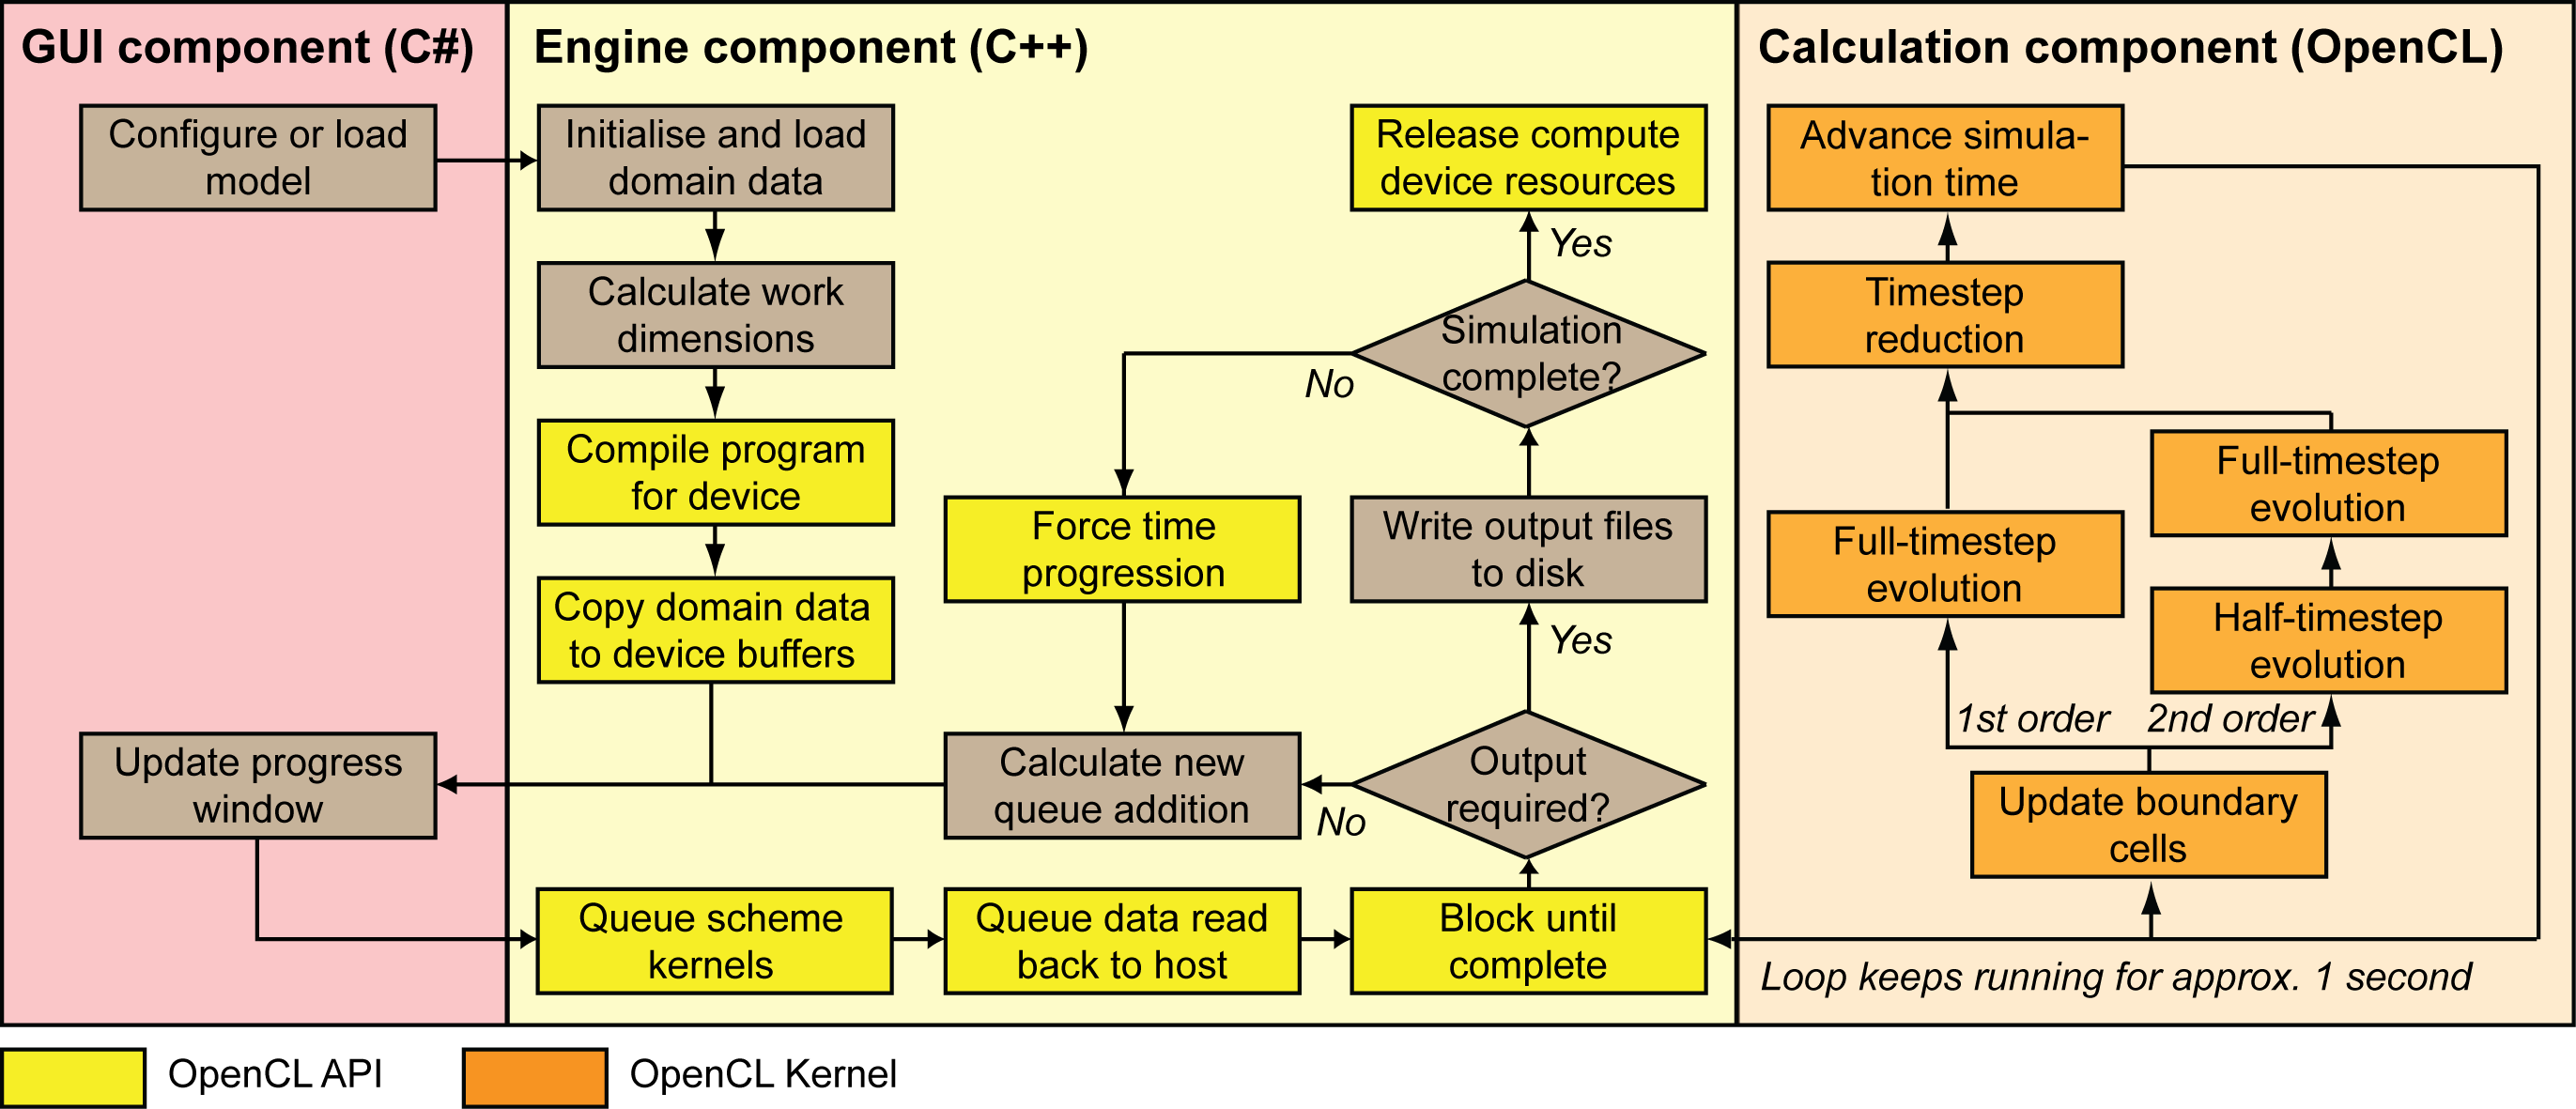
\includegraphics[width=1.0\textwidth]{HiPIMS_Structure_NoVis.png}
\caption{Flowchart of the software processes indicating which components are OpenCL kernels or API calls.}
\label{HiPIMS_Structure_NoVis}
\end{figure*}

Moving data from the main system memory (RAM) to a GPU device is an expensive operation \citep[see recommendations in][]{AdvancedMicroDevicesInc2011,NVIDIACorporation2009}. Cell data is only moved periodically for output files, and the numerical scheme is otherwise permitted to run in a loop for approximately one second before a small amount of data is transferred to update the user on the progress of the simulation. This process is represented in \ref{HiPIMS_Structure_NoVis}. No vendor-specific optimisations were made, as the authors' intentions were to create a system appropriate for use with any of the mainstream vendors' hardware, most notably NVIDIA, AMD and Intel. The compiler is instructed to adhere to all of the appropriate IEEE standards for floating-point arithmetic (i.e. accurate square root operations, treatment of denormals, etc.).

A regular Cartesian grid is used to represent the domain, whereby transient state variables are stored in a four-element vector and constant values (bed elevation and friction coefficients) require two further elements. This means 48 bytes or less are required per cell. Considering further constraints imposed on the size of a single memory allocation, the software is presently limited to 50 million cells for current hardware offering up to 6GB of memory.

A two-stage reduction process (\ref{HiPIMS_Reduction}) is used to identify the largest permissible timestep within the domain: cells are sampled with a regular stride and recursive binary comparisons used to provide a single value which is carried forward to a much smaller array. This is examined in the second stage when incrementing the overall simulation time. The reduction process ensures processors perform sufficient work to mask the considerable latency introduced by transferring data from a GPU's globally-accessible memory to compute unit-specific registers. A variety of raster formats are supported for importing and exporting domain data, initial conditions, and periodic output. 

\begin{figure*}[tpb]
\centering
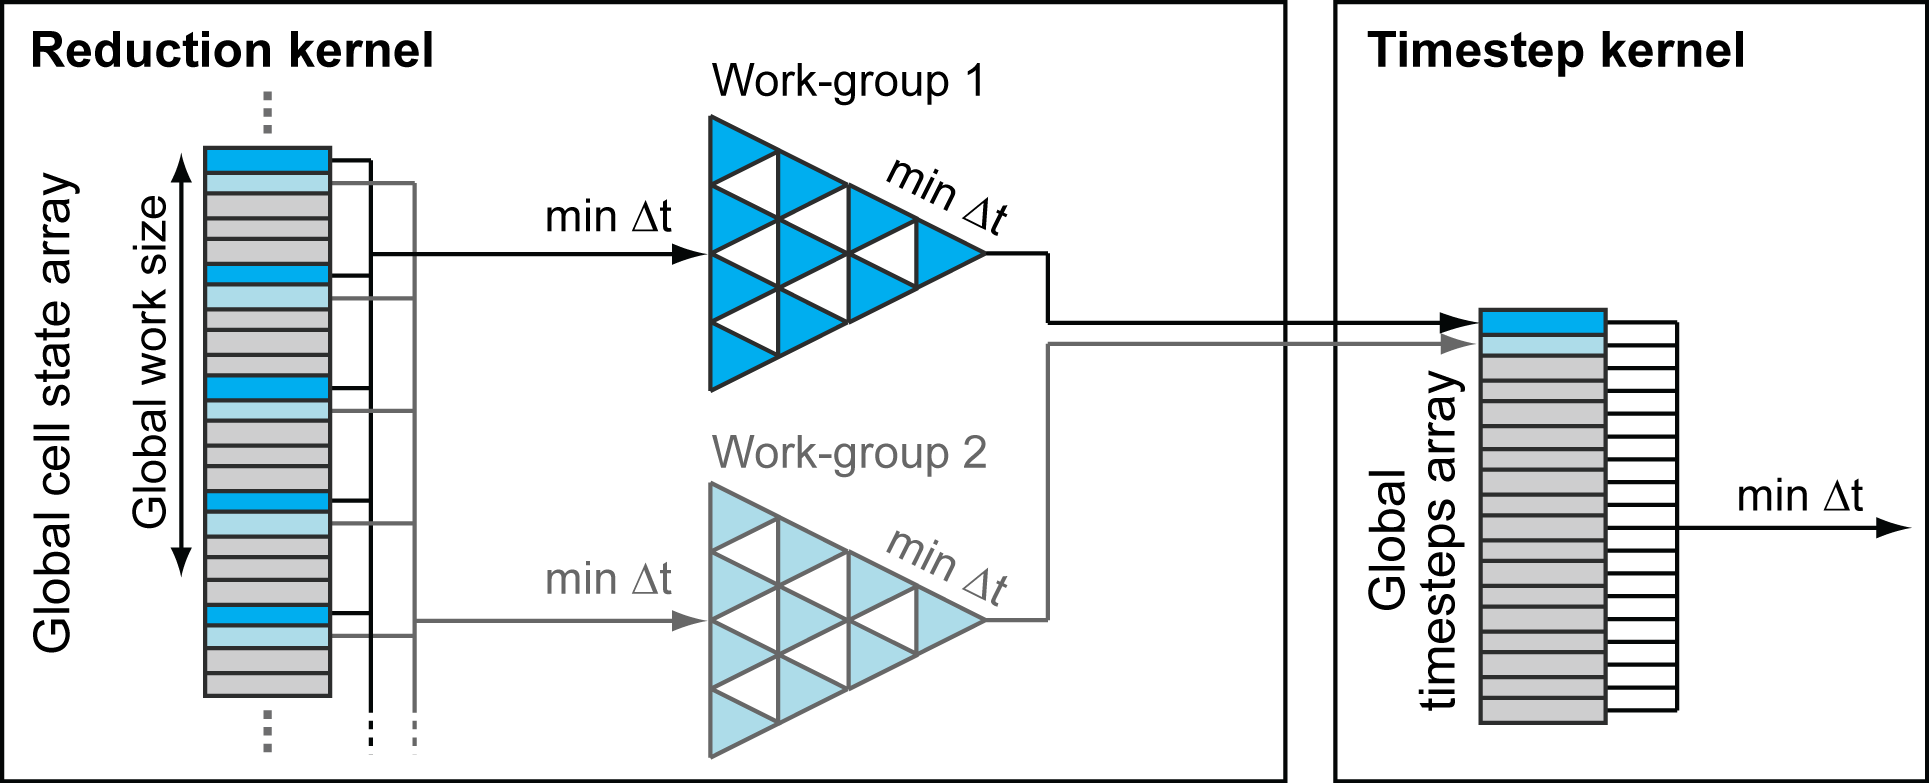
\includegraphics[width=0.8\textwidth]{HiPIMS_Reduction_Colour.png}
\caption{Representation of a two-stage reduction process with a global stride of six (stride in reality would be much larger) performing a series of binary comparisons to create a smaller array of potential values.}
\label{HiPIMS_Reduction}
\end{figure*}

\section{Results and discussion}

The aforementioned software has been applied to inundation simulations in Glasgow and Thamesmead, both in the United Kingdom. The first represents a standard test-case to allow comparison with commercially-available hydraulic modelling packages. The latter represents a much larger-scale test that would be burdensomely slow without GPU acceleration. The Courant number is 0.5 for both cases. Both cases are simulated using an Intel Xeon E5-2609 CPU device \citep{Intel_12}, AMD FirePro V7800 GPU \citep{AdvancedMicroDevicesInc2010a}, and NVIDIA Tesla M2075 GPU \citep{NVIDIACorporation2011}.

\subsection{Glasgow}

The UK Environment Agency commissions a report periodically examining the differences in results, suitability and performance of different 2D hydraulic modelling packages. One of the more complex test-cases therein is a short hypothetical flood event occurring as a combination of both a point inflow and uniform precipitation in the area surrounding Cockenzie Street, Glasgow. The test was performed in accordance with \citet{Pender2010} and \citet{Pender2013}, simulating a 5-hour period.

The inflow hydrograph and hyetograph are given in \ref{Glasgow_Inflows}. The digital terrain model (DTM) is shown in \ref{Glasgow_DTM} alongside the location of the point inflow at $(264896, 664747)$. Data was supplied at 0.5m resolution but has been resampled to 2m to allow comparison with published results for other software. The computational domain contains 97,083 cells. A uniform Manning coefficient of 0.05 is used everywhere except for roads and pavements where a value of 0.02 is assigned. Closed boundary conditions are applied around the extremity of the domain. 

\begin{figure*}[tpb]
\centering
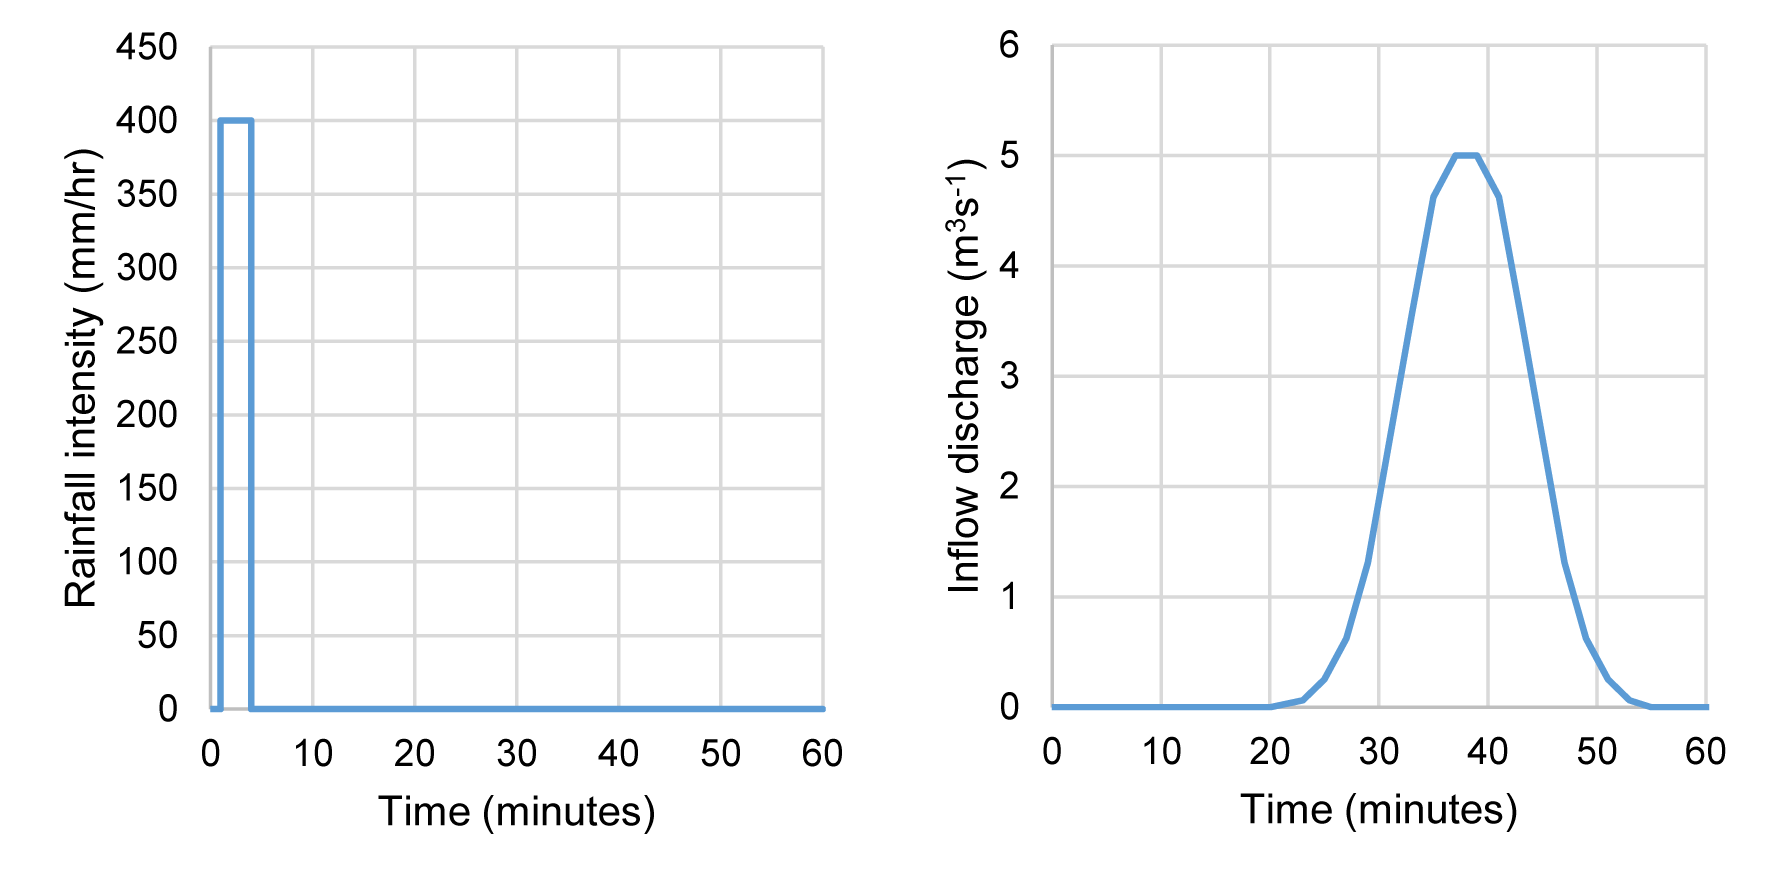
\includegraphics[width=0.75\textwidth]{Glasgow_Inflow.png}
\caption{(a) Uniformly distributed rainfall hyetograph; (b) volumetric discharge at the inflow point.}
\label{Glasgow_Inflows}
\end{figure*}
\begin{figure*}[tpb]
\centering
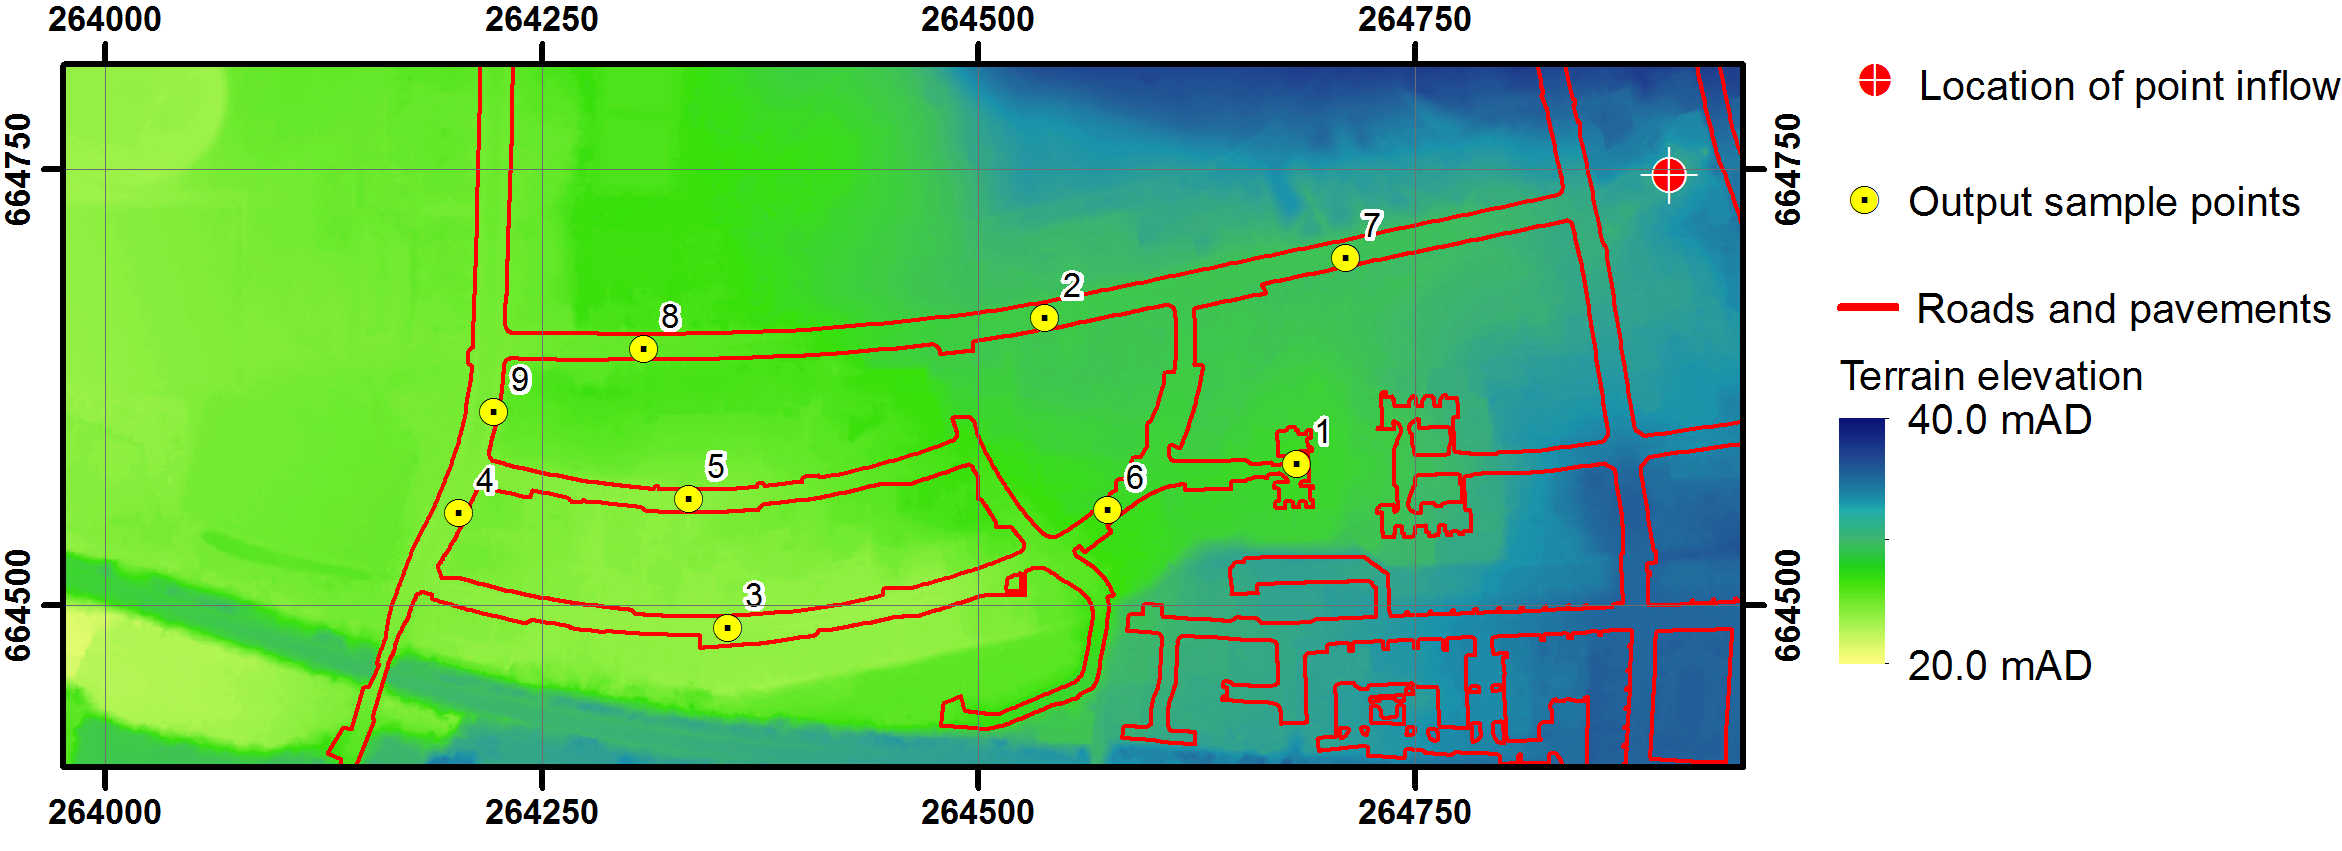
\includegraphics[width=1.0\textwidth]{Glasgow_DTM.png}
\caption{The surface elevation for a 0.39 km$^{2}$ area of Glasgow with the inflow location indicated and the position of 9 output sample points.}
\label{Glasgow_DTM}
\end{figure*}

Simulations were carried out using 32- and 64-bit floating-point arithmetic (i.e. single- and double-precision). 32-bit arithmetic introduced significant errors in mass conservation for the given numerical scheme and resulted in timesteps of approximately 0.1s. This is believed to be caused by the lack of numerical resolution for the small depths by which unit-width discharge is divided to give velocities. The typical timestep with 64-bit arithmetic is approximately 0.3s. This difference largely negates the performance benefits that are normally achievable with reduced precision arithmetic for both GPUs and CPUs, and furthermore has implications for any other simulations in which extremely shallow flows might be expected. Results presented hereafter are for 64-bit simulations except where indicated.

The maximum depths recorded per cell at the end of the simulation are displayed in \ref{Glasgow_MaxDepths} at 0.2m intervals. In addition water levels and velocities were output at 9 different points; levels are shown in \ref{Glasgow_PointGraphs} while velocities are omitted for brevity. The maximum depths and timeseries data are consistent with results produced by other software, and close to those of other finite-volume software packages in particular. Small differences are discernible but all fall within the ranges of results presented in \citet{Pender2010}.

\begin{figure*}[tpb]
\centering
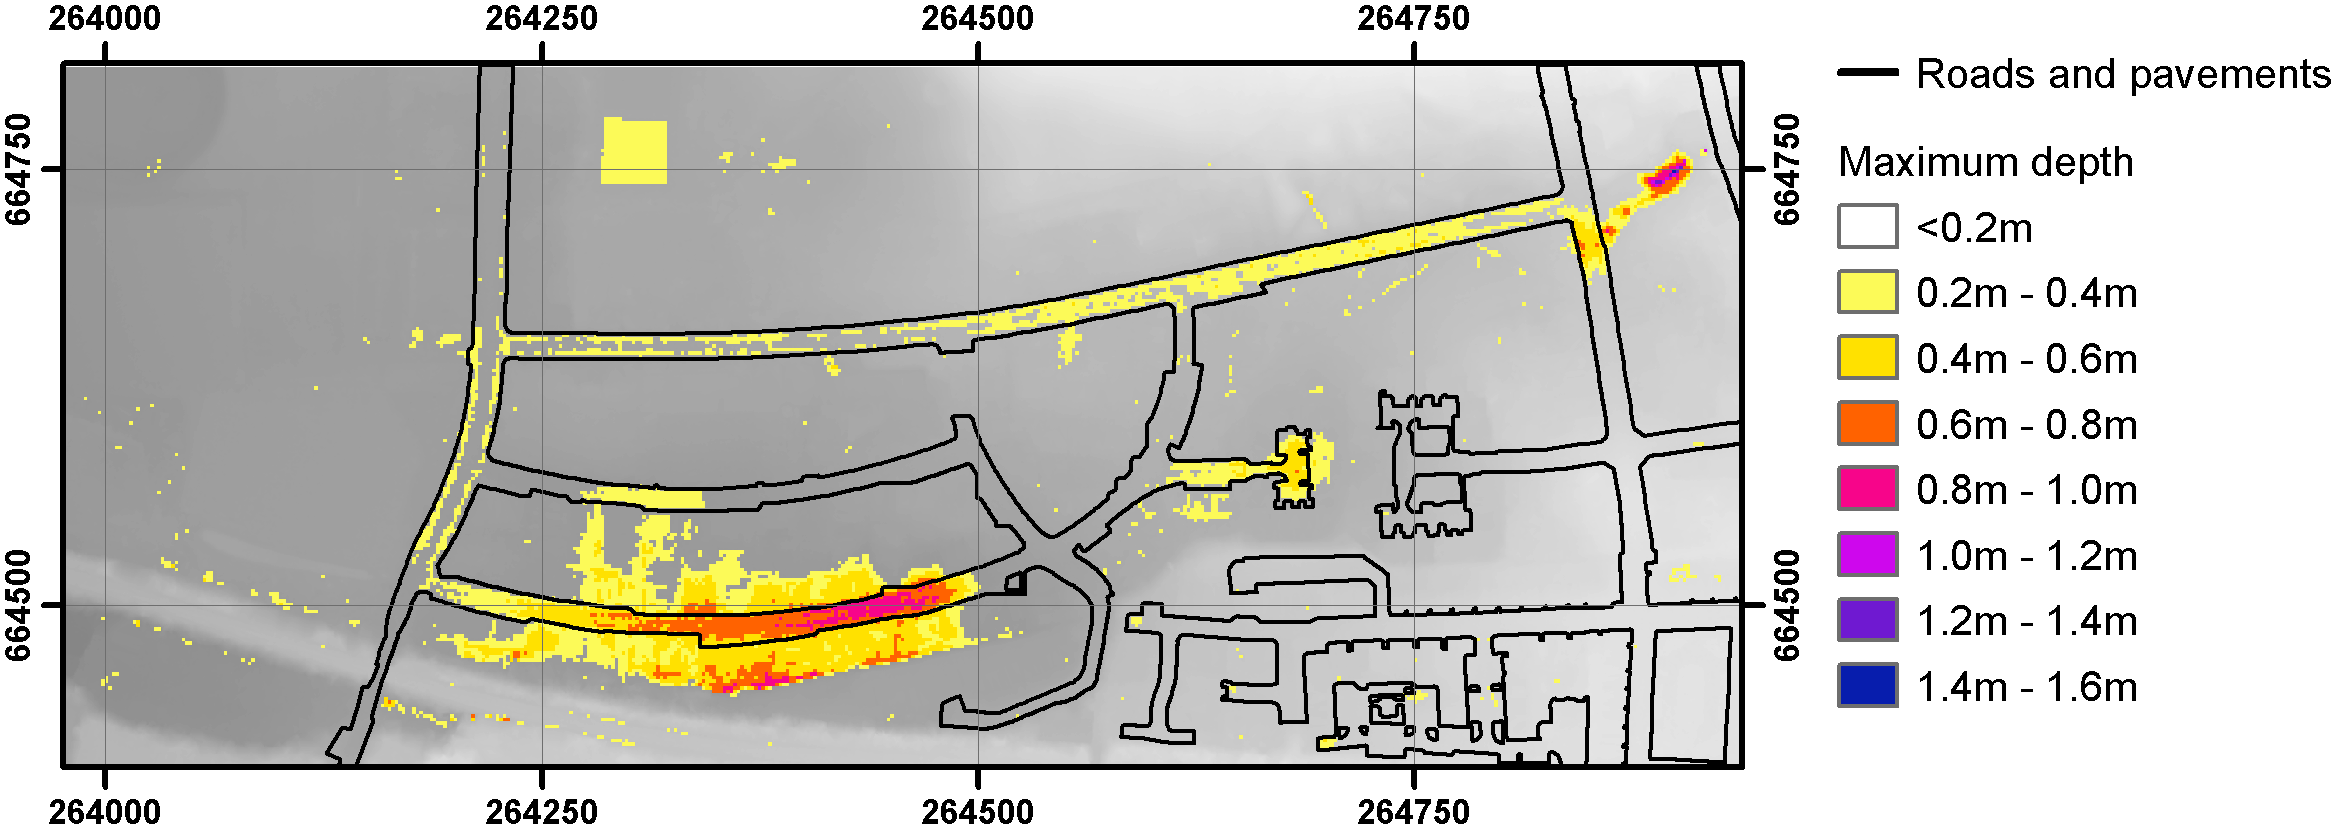
\includegraphics[width=1.0\textwidth]{Glasgow_MaxDepths.png}
\caption{Maximum water levels observed per cell after 5 hours, shown at 0.2m intervals.}
\label{Glasgow_MaxDepths}
\end{figure*}
\begin{figure*}[tpb]
\centering
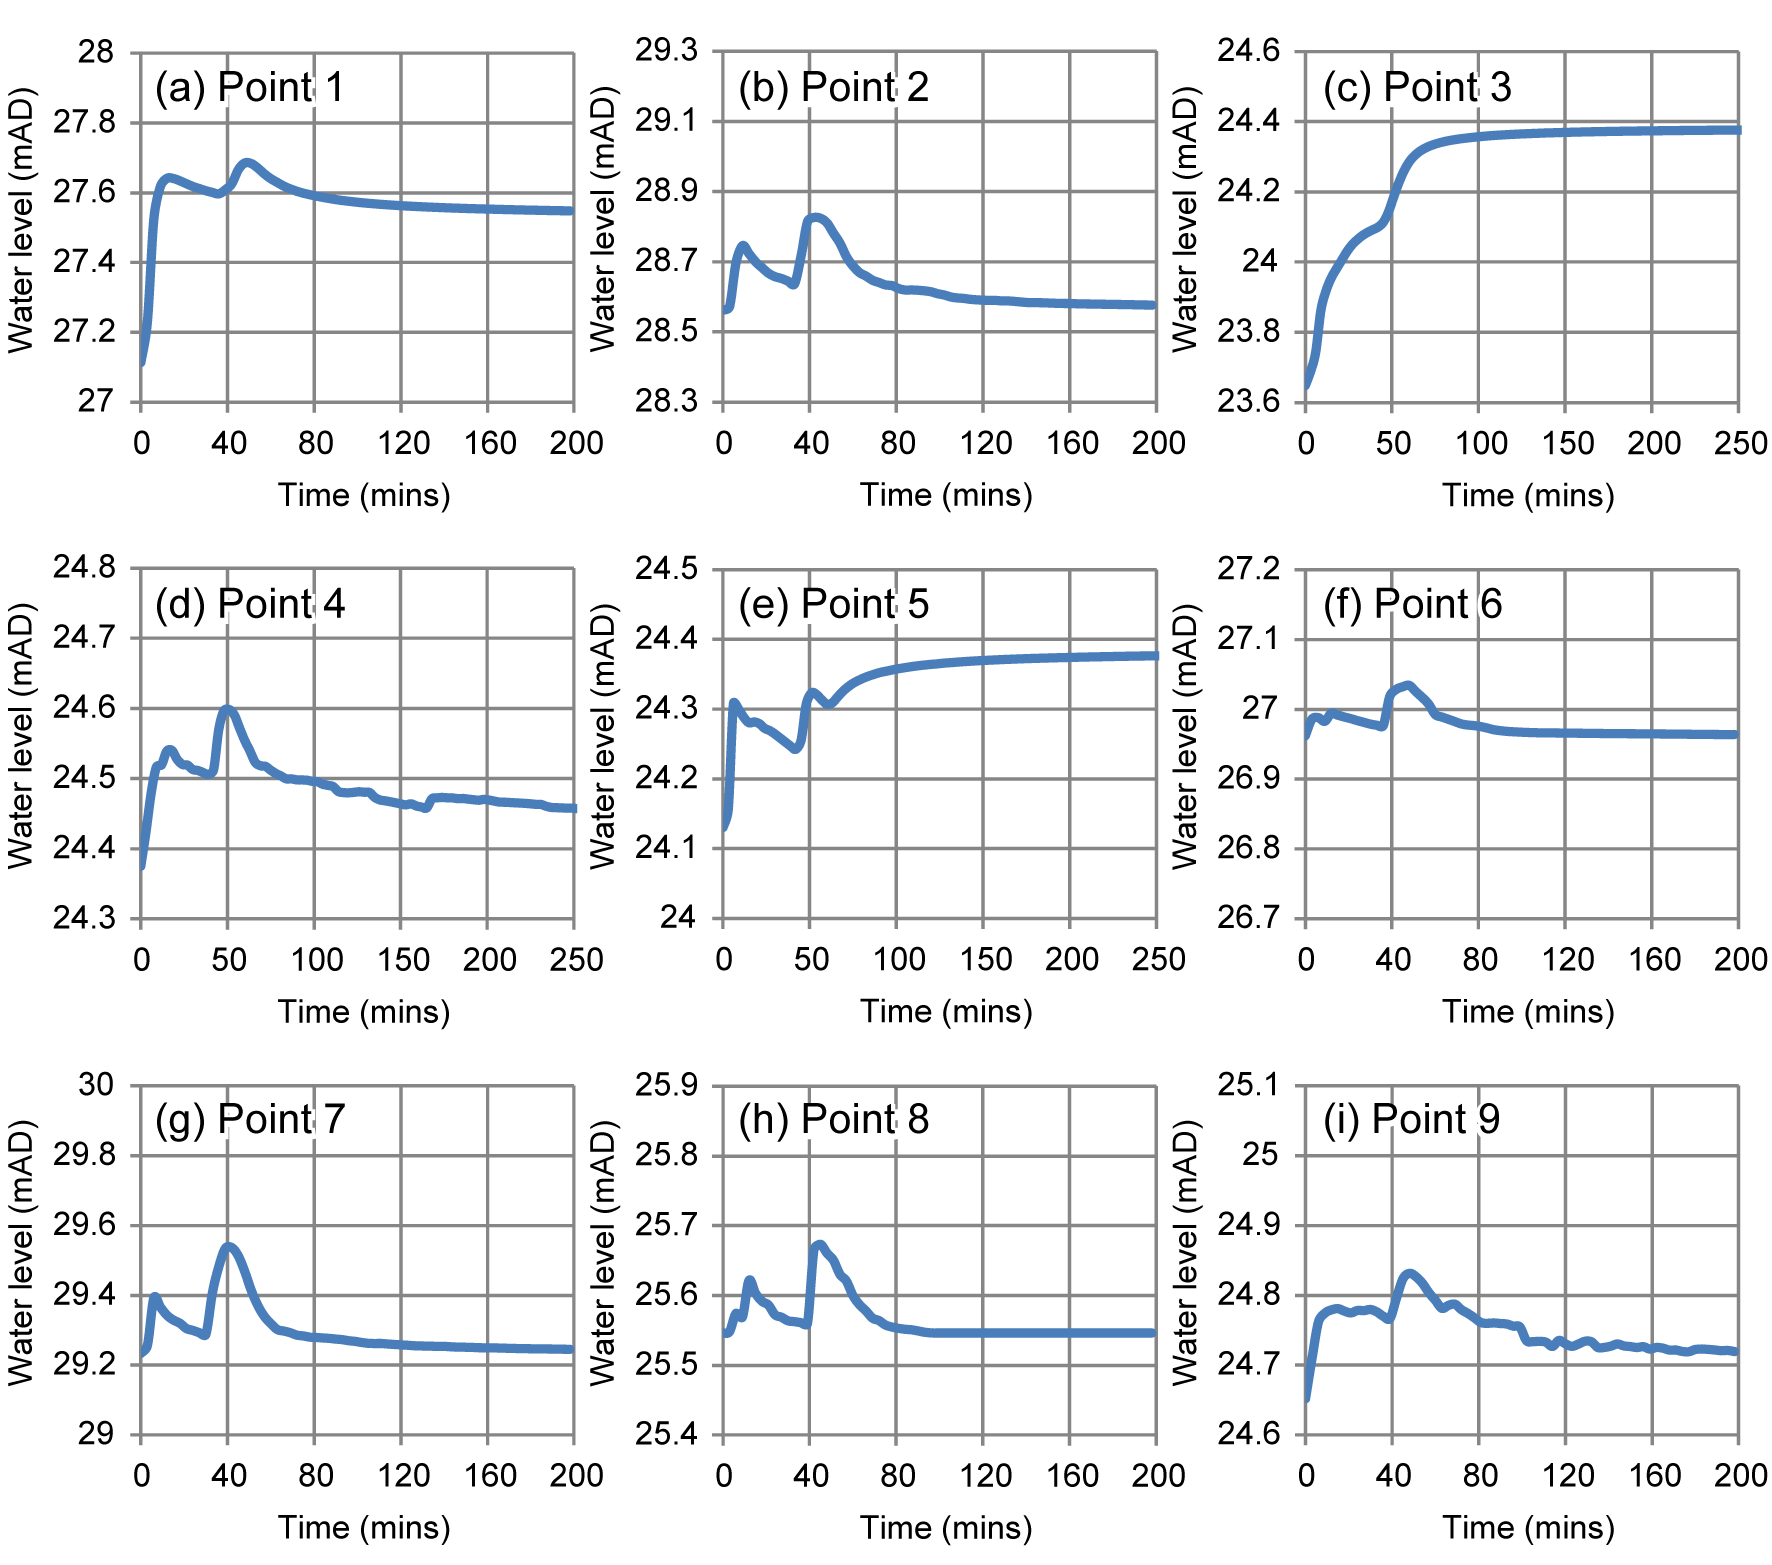
\includegraphics[width=0.8\textwidth]{Glasgow_PointGraphs.png}
\caption{Changes in recorded water levels above datum recorded at 9 different sample points in the domain. The location of the sample points is given in \ref{Glasgow_DTM}.}
\label{Glasgow_PointGraphs}
\end{figure*}

The simulation correctly represents the double-peaked nature of the event from intense rainfall and subsequent surcharging of a sewer, with the second peak at point 7 shortly after the surcharging peaked at 38 minutes. The results are generally free of oscillations, except for some small oscillations at point 9 which may be unphysical. At point 2 there is some discrepancy among models as to when the water levels settle after both peaks have passed; the results presented herein suggest this occurs after approximately 120 minutes, which is consistent with the results for the comparable numerical scheme employed in TUFLOW FV. At point 3 the second peak begins at approximately 50 minutes, which is consistent with almost all of the software in \citet{Pender2013}. At point 6 the second peak is predicted to occur at around 27.05 mAD, which is higher than many of the other software but there is significant variation across software at this point, ranging from 26.95 to 27.08 mAD. The final flood depths correspond to the areas which were predicted by the majority of software tested in \citet{Pender2013}; clearly a shock-capturing scheme is not necessary to accurately predict the final extent, but can have a marked effect on the progression of the flood wave, localised flow dynamics and arrival timing, all of which could be significant factors in assessing flood risk and crucial in issuing flood warnings. It cannot be asserted as to which software is most accurate as the event and inflow data is hypothetical, however the software herein captures the same behaviour as comparable finite-volume codes solving the full shallow water equations. Small differences in the methods for solving the equations and implementation of boundary conditions can result in significant differences: treatment of wet-dry fronts, frequency of mass addition for precipitation, rounding or smoothing in the consideration of topography, and mechanism for considering the Manning coefficient are believed to be most significant in this instance.

\begin{table*}[pb]
\small
\centering
\caption{Simulation run-times for Glasgow in minutes using three different processing devices.}
\label{GlasgowPerformance}
\begin{tabular}{p{0.2\textwidth}p{0.2\textwidth}p{0.2\textwidth}p{0.2\textwidth}}
\hline
\raggedright{Floating-point arithmetic resolution}	& \raggedright{CPU Intel Xeon E5-2609} & \raggedright{GPU AMD FirePro V7800} 		& GPU NVIDIA Tesla M2075 \\
\hline
32-bit 							& 9.05					& 2.47					& 1.98				\\
64-bit 							& 9.45					& 2.67					& 2.88				\\
\hline
\end{tabular}
\end{table*}

The run-times for the simulation using three different processing devices are presented in \ref{GlasgowPerformance}. It is important to note however that the domain for this test-case is too small to fully exploit the weak scaling in GPUs. Nonetheless the times represent a significant reduction on those in \citet{Pender2010} and \citet{Hunter2007}, with both CPU and GPU computation, despite the use of an explicit numerical scheme and Godunov-type scheme. Compared to figures reported for the same test in \citet{Pender2013}, the software presented herein is slightly slower than some comparable GPU software (e.g. 1.40 minutes for TUFLOW GPU), which may in part be a result of using OpenCL parallelisation, where there is some evidence to suggest memory transfers and dispatch overheads could be slightly higher than CUDA \citep[e.g.][]{Karimi2010}. The performance results cannot be directly compared however as different hardware was used for each software. Moreover, the CUDA and OpenCL APIs have subtle but important differences between implementations, such as the non-standard blocking behaviour of \texttt{clEnqueueNDRangeKernel} in NVIDIA's implementation of OpenCL. Comparison is also difficult as diffusion approximation codes can be expected to exhibit poor computational efficiency at 2m resolution because of a more severe timestep constraint.

\subsection{Thamesmead}

\begin{figure*}[tpb]
\centering
    \begin{subfigure}[t]{0.5\textwidth}
        \centering
        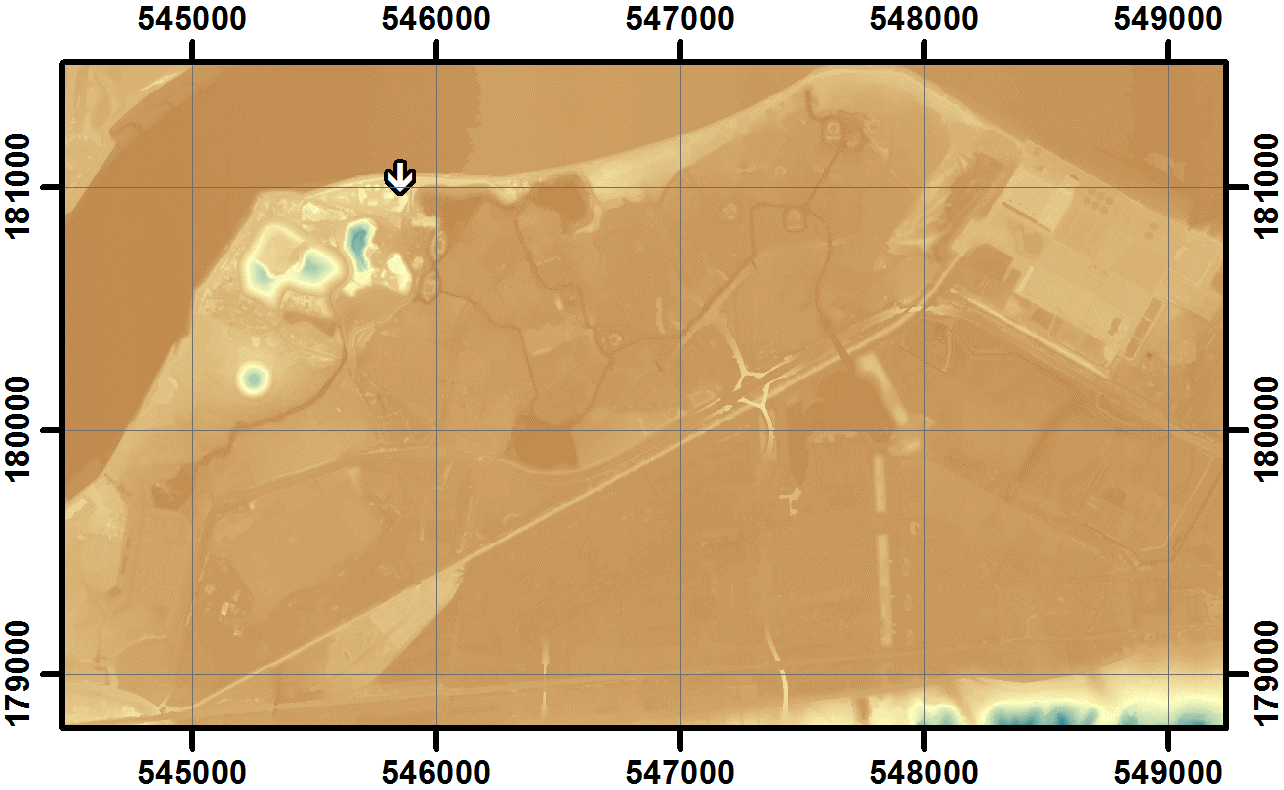
\includegraphics[width=1.0\textwidth]{Thamesmead_DTM.png}
        \caption{Digital terrain model (DTM) and inflow location for Thamesmead}
    \end{subfigure}%
    ~ 
    \begin{subfigure}[t]{0.5\textwidth}
        \centering
        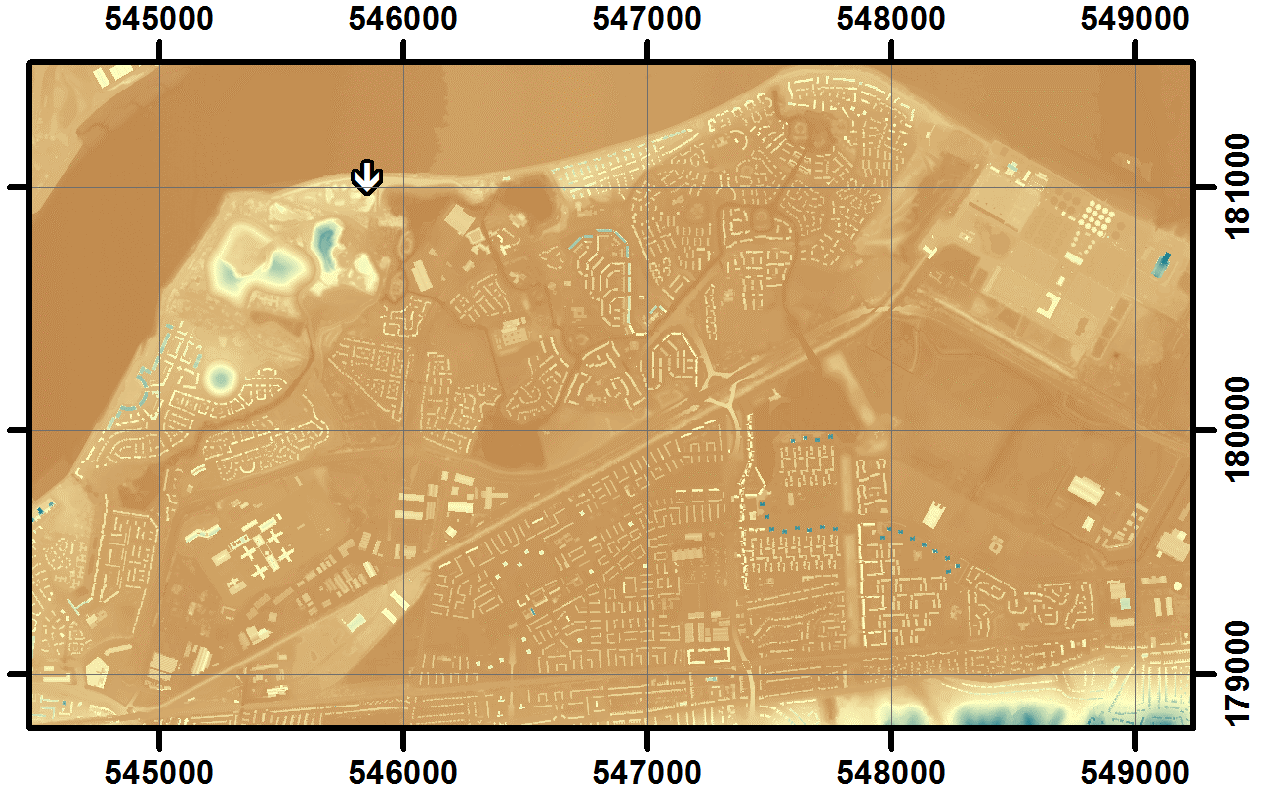
\includegraphics[width=1.0\textwidth]{Thamesmead_DEM.png}
        \caption{Digital elevation model with buildings included (DEM).}
    \end{subfigure}

    \begin{subfigure}[t]{0.7\textwidth}
        \centering
        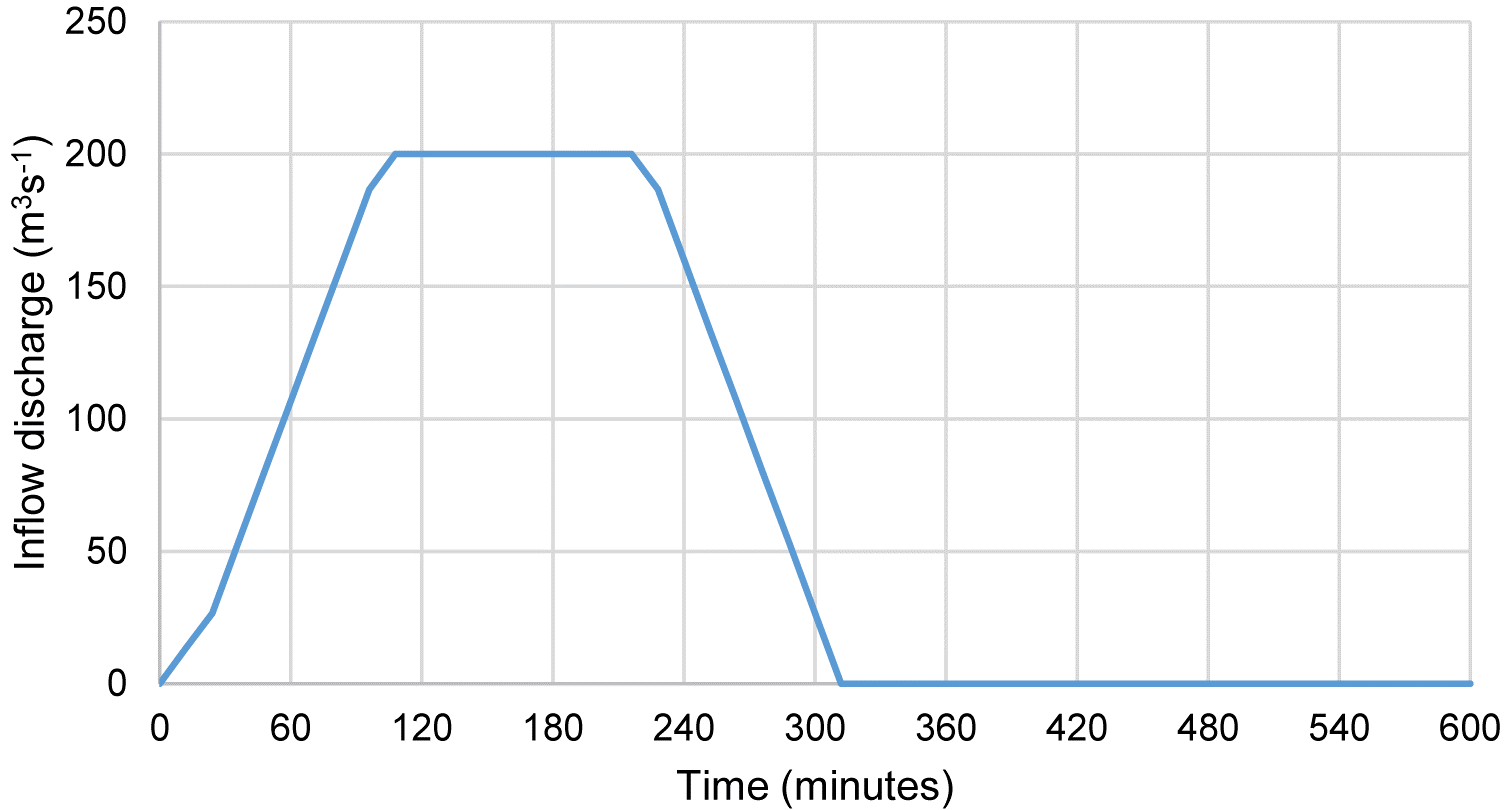
\includegraphics[width=1.0\textwidth]{Thamesmead_Inflow.png}
        \caption{Volumetric discharge at the breach location.}
    \end{subfigure}
\caption{Boundary conditions and topography used in Thamesmead simulations.}
\label{Thamesmead_Conditions}
\end{figure*}

The Thamesmead district of South London is located downstream of London's main flood defence, the Thames Barrier. The area is low lying but was heavily developed in the 1960s. Flood risk is posed by storm surges or a failure in the defence wall, with the area previously inundated in the North Sea Surge of 1953. A hypothetical breach in the defences is considered here, through which over 2,500,000m$^{3}$ of water enters the area with the hydrograph and entry point indicated in \ref{Thamesmead_Conditions}. A 10-hour period is simulated, allowing the water to continue spreading through the computational domain. 

The same hypothetical event is considered by \citet{Liang2008a}, \citet{Liang2010a}, and \citet{Vacondio2012}. These studies used a 10m resolution grid of 360,000 cells, whereby buildings and vegetation were removed from LiDAR altimetry data to create a digital terrain model (DTM). The software presented herein allows us to go further. Updated datasets were created using a 2007 survey, and the resulting DTM and elevation model with buildings included (DEM) are shown in \ref{Thamesmead_Conditions} at 2m resolution with 9,013,004 cells. As previously a uniform Manning coefficient of 0.035 is applied across the domain. Cells within and north of the River Thames are excluded from computation. Transmissive boundary conditions are imposed at the domain edges. The final volume error is \textless1\% of the inflow volume for all Thamesmead simulations discussed.

\begin{figure*}[tpb]
\centering
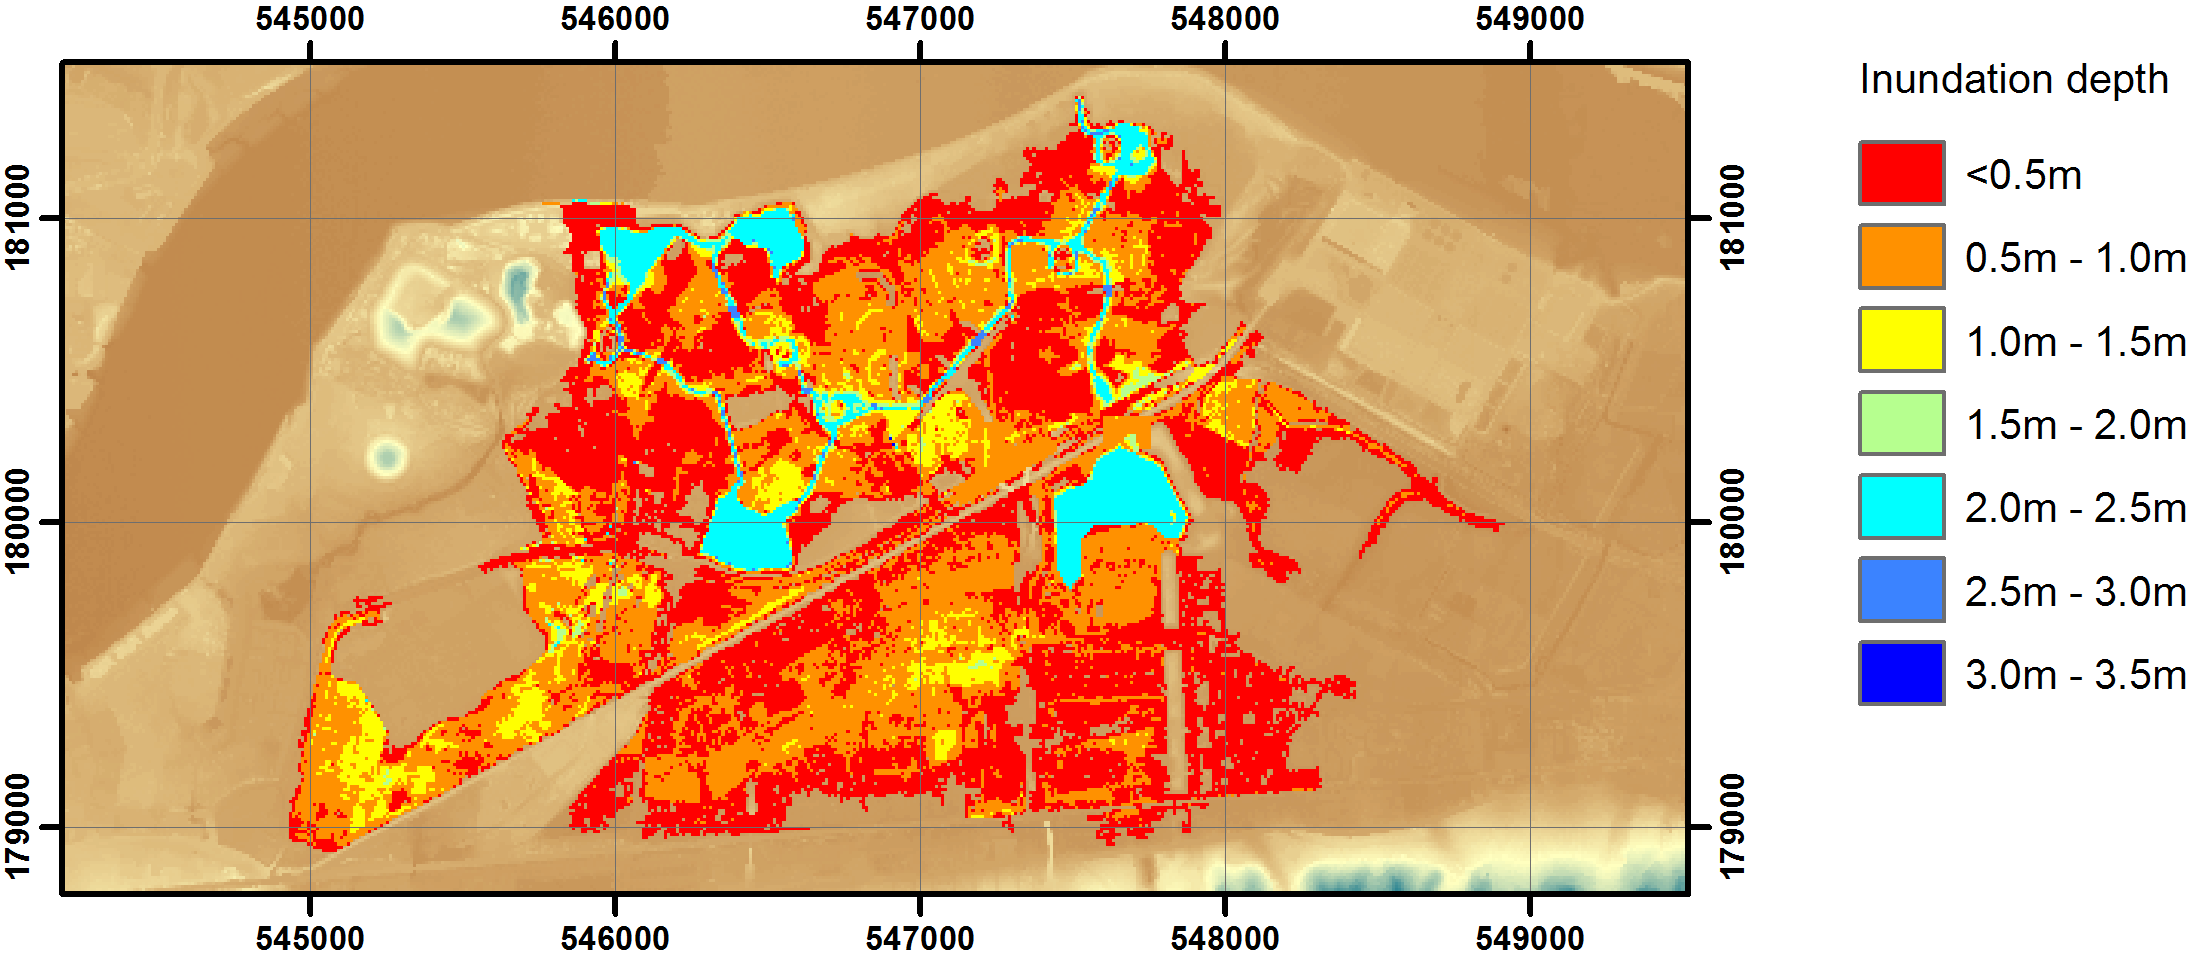
\includegraphics[width=1.0\textwidth]{Thamesmead_10m_Comparison.png}
\caption{Inundation results after a 10-hour period for the 10m resolution DTM used in Liang (2010).}
\label{Thamesmead_10m_Comparison}
\end{figure*}

We start by attempting to reproduce the simulation previously explored in literature with a 10m DTM, in order to further validate the model. The inundation results are presented in \ref{Thamesmead_10m_Comparison}, where only minimal disagreement can be identified against the results in \citet{Liang2010a}. This stems from differences in treatment of inflow boundary conditions for the new software. It can clearly be seen that a lesser flood extent is found with the new DTM in \ref{Thamesmead_Inundation} for the same resolution. The updated terrain model depicts a deeper network of canals and lakes, offering increased storage. 

Simulations were undertaken using both 32-bit and 64-bit floating-point arithmetic. Results presented are for 64-bit unless otherwise indicated. Whilst the average error in depth introduced by 32-bit arithmetic is small, the localised errors are in some cases unacceptably large. Errors were more pronounced at 10m resolution with the DEM; the average error exceeded 0.1m and the largest error was 0.98m. By contrast the average errors for all simulations at 5m and 2m resolution were \textless 0.01m. The magnitude of these errors is in part a function of the numerical scheme employed, although it would not be entirely surprising if coarse resolutions are more sensitive to numerical resolution given the larger volume affected by the same change in depth. Further research is required. 

The final extent and inundation depth for the three resolutions and two elevation models employed are shown in \ref{Thamesmead_Inundation}. The building layout is unusual in Thamesmead, with numerous connected networks of buildings. Small tunnels and alleyways allow for pedestrian access, and the elevation models have been adjusted to ensure these are present as a flow pathway. These passages are small however, hence the buildings can be expected to reflect a large volume of the flow impacting them; this is confirmed by the results obtained. Inclusion of buildings results in an increased inundation in the west of the domain. Spatial resolution also has a substantial impact on the flood extent. \ref{Thamesmead_Velocities} shows the magnitude of the velocities after six hours, with the highest velocities present at the highest resolutions where narrow gaps are clearly resolved, concentrating flow to alleyways and streets. As a consequence flood progression is more rapid at higher resolutions. In this case, coarse resolutions may result in underestimation of flood extent.

Additional simulations were run for each grid resolution with different Manning's $n$ values from 0.01 to 0.09 at 0.02 increments, giving 30 simulations in total. This allows the sensitivity to parameterisation to be assessed. The minimum and maximum extent of flooding after 10 hours across the calibration range is shown in \ref{Thamesmead_Inundation}. As expected, a lower Manning's $n$ results in a larger area of inundation by the end of the simulation. Consistent with the findings of \citet{Yu2006}, coarser grid resolutions exhibit lower sensitivity to Manning's $n$, while there is a substantial range in final extent for both the DEM and DTM at 2m resolution. This is unsurprising given the higher localised velocities at fine grid resolutions. Low sensitivity to parameterisation at coarse grid resolutions is not a justification for using these resolutions however, as the difference in inundation from coarse to fine resolution grids far exceeds the scope of influence any parameterisation might have. Consequently there is a clear need for sub-grid scale representation of topographic features, dynamically adaptive grids, or use of high-resolution grids throughout. 

\begin{figure*}[tpb]
\centering
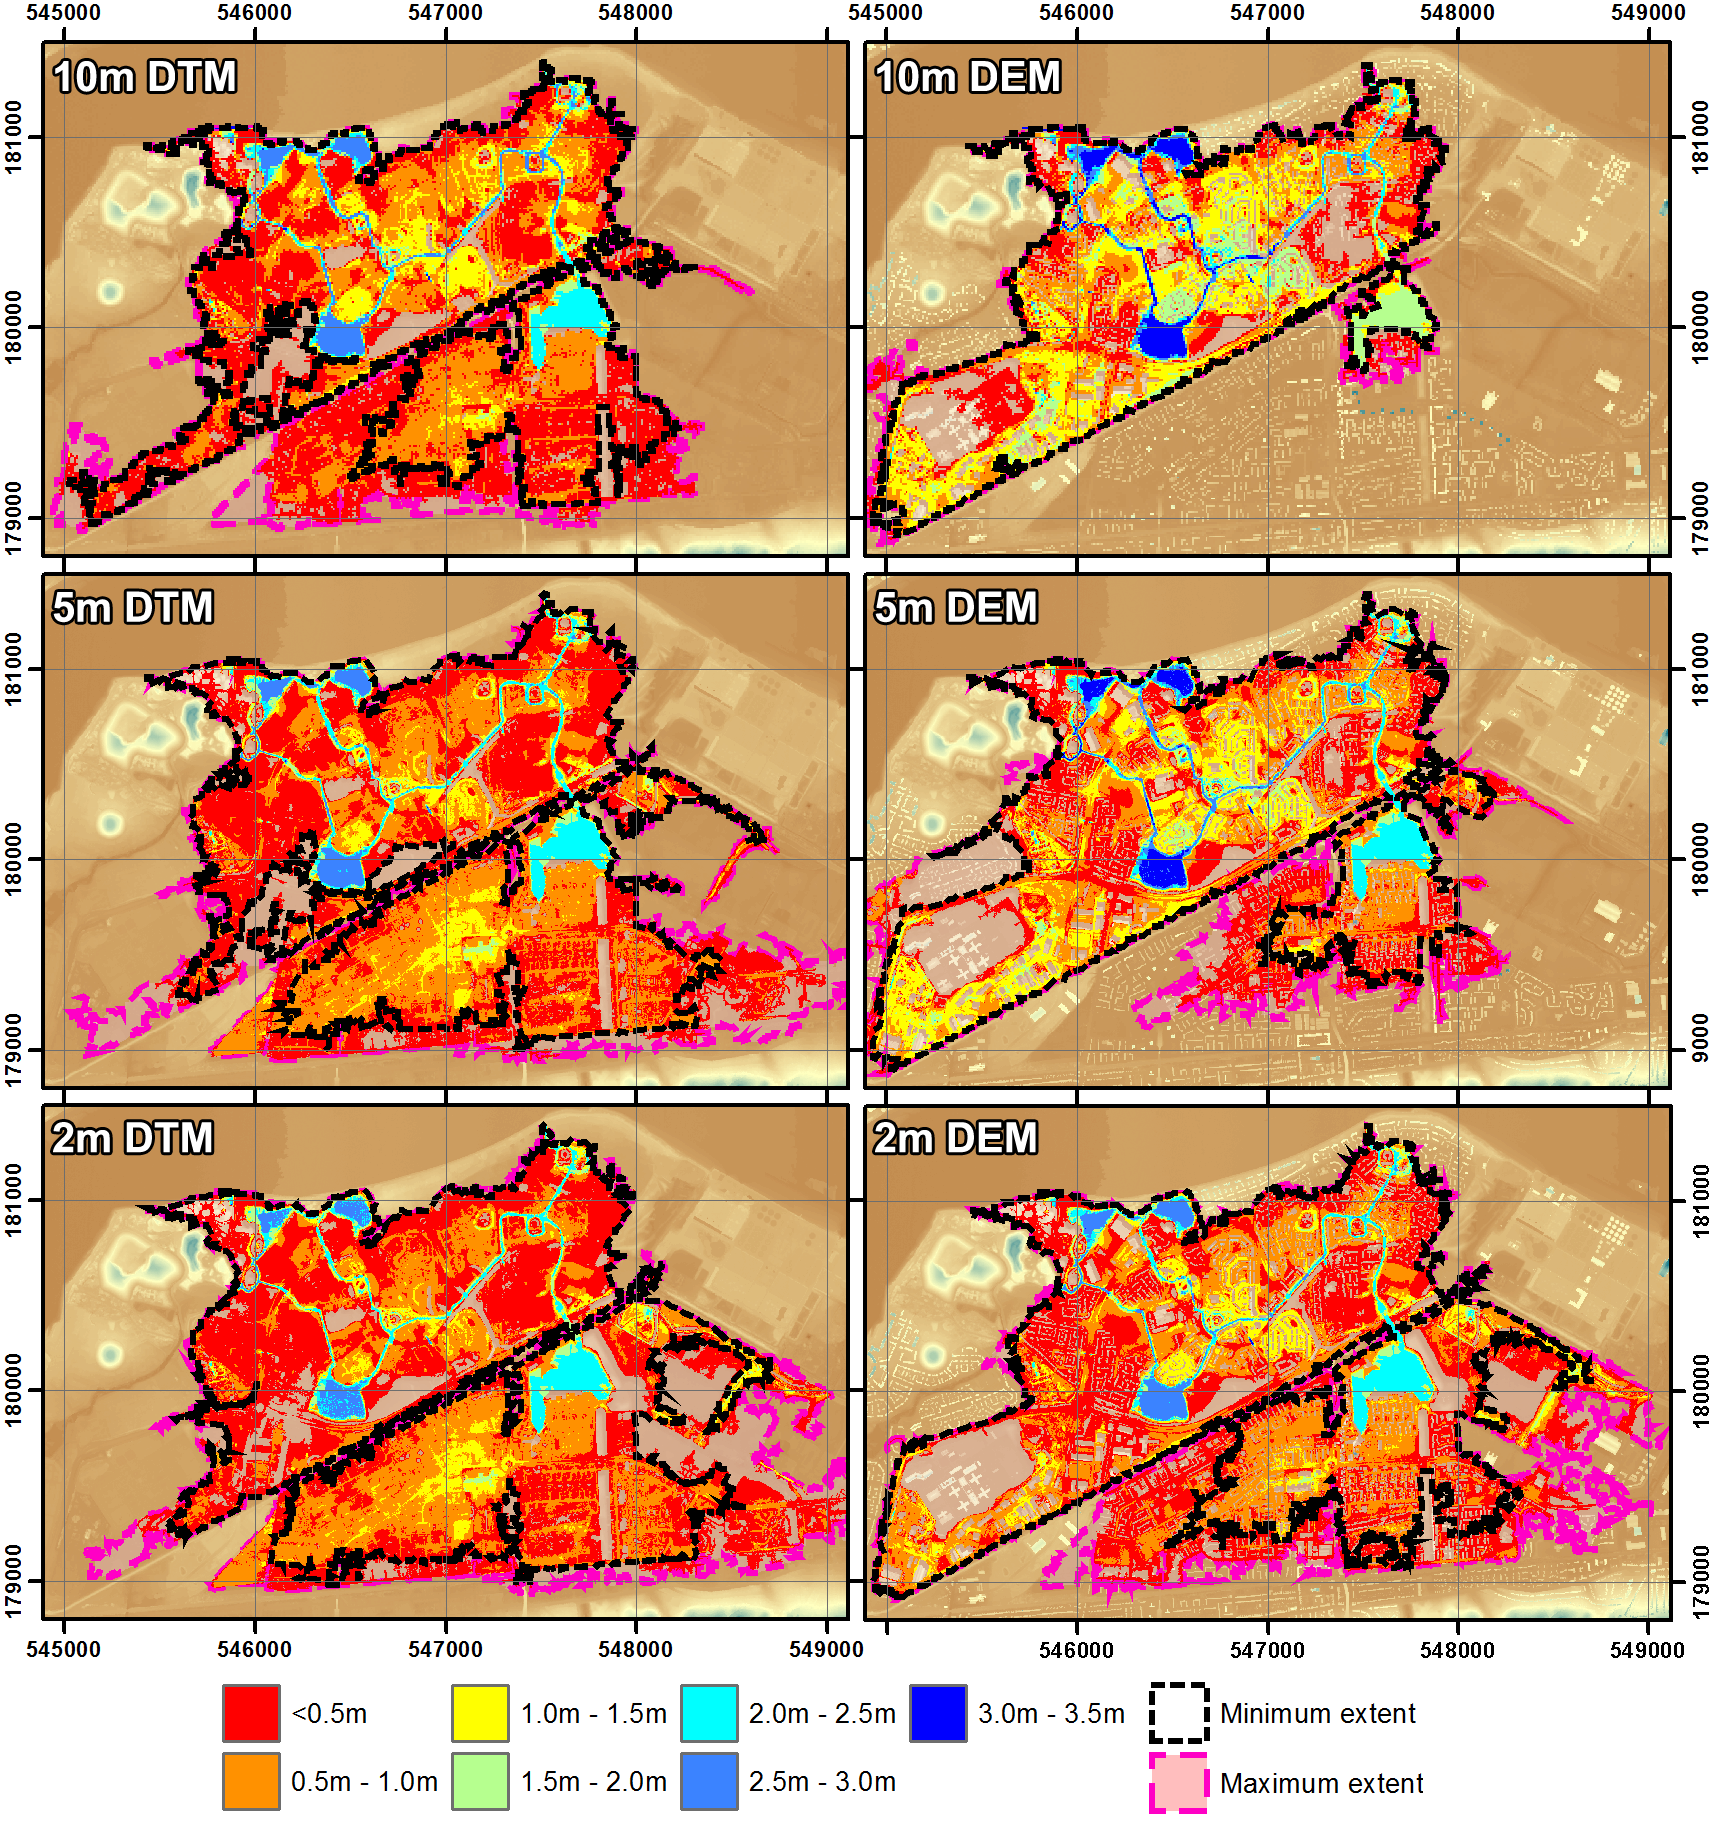
\includegraphics[width=1.0\textwidth]{Thamesmead_AllDepths.png}
\caption{Inundation results after a 10-hour period using DEM and DTM at different spatial resolutions, and the minimum and maximum inundation extents with Manning values from 0.01 to 0.09.}
\label{Thamesmead_Inundation}
\end{figure*}
\begin{figure*}[tpb]
\centering
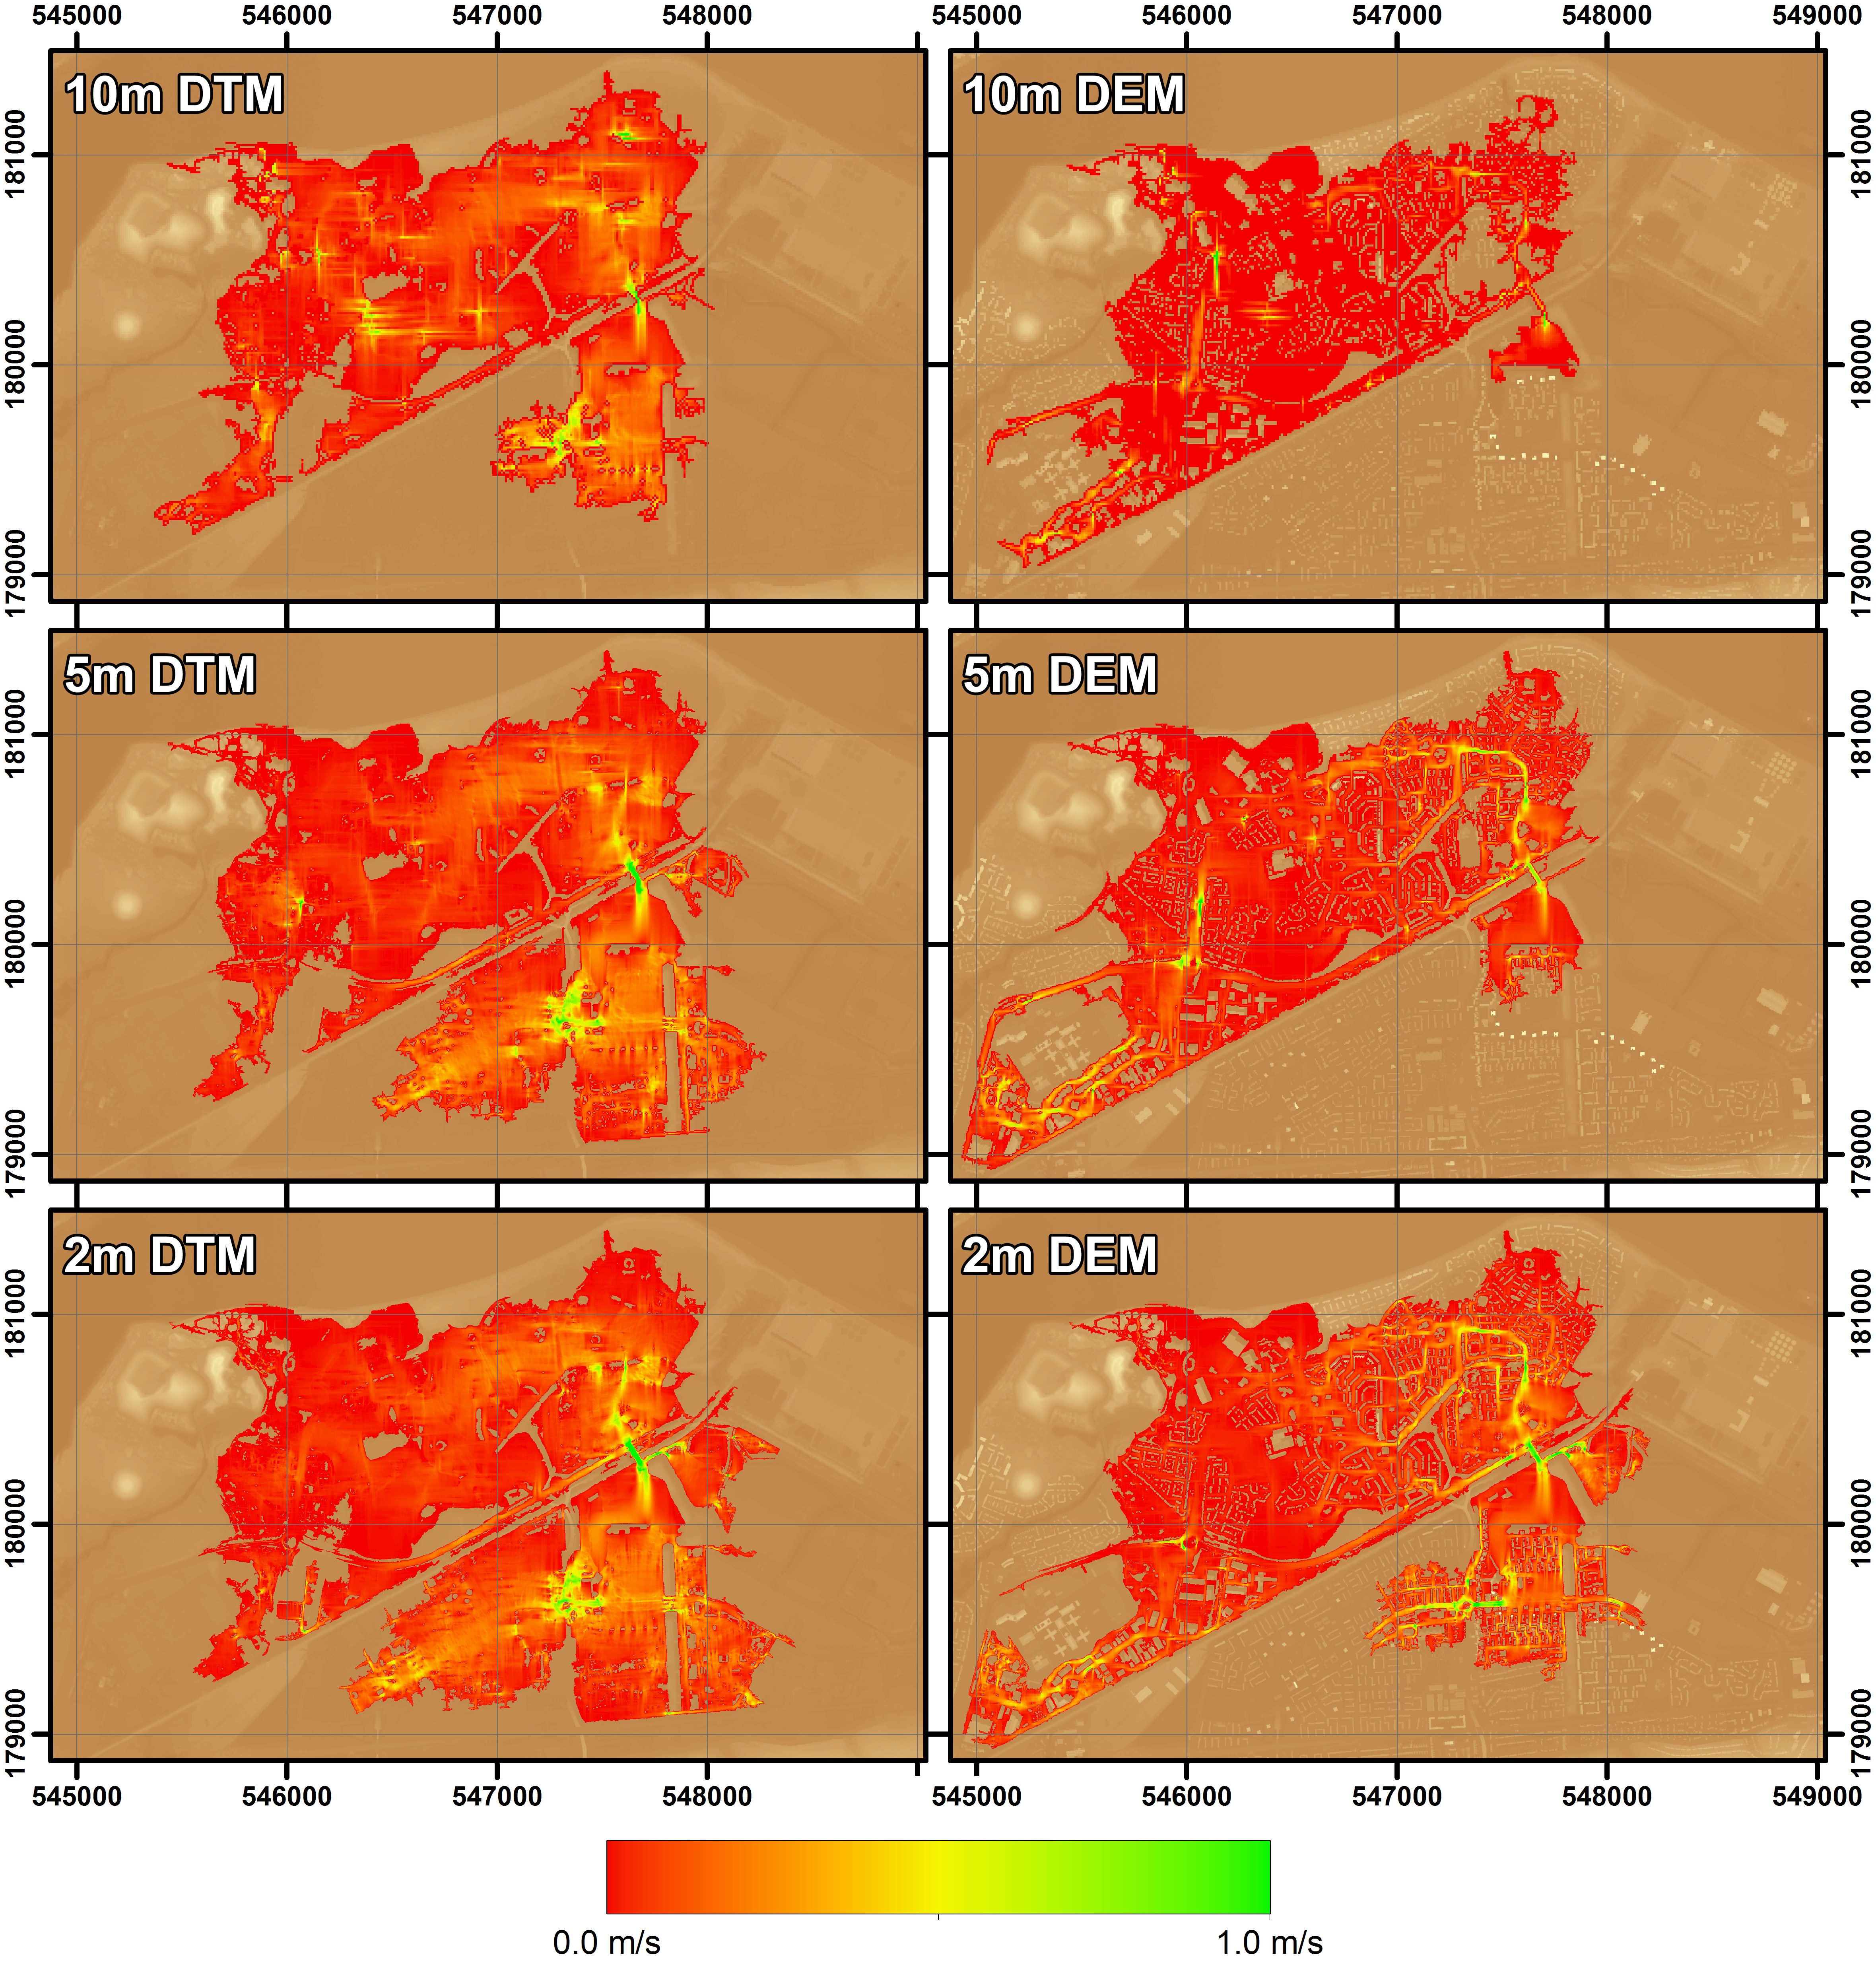
\includegraphics[width=1.0\textwidth]{Thamesmead_AllVelocities.png}
\caption{Magnitude of velocities at 6 hours using DEM and DTM at different spatial resolutions. }
\label{Thamesmead_Velocities}
\end{figure*}

The high-velocity nature of this hypothetical event contributes to the higher sensitivity, in contrast to studies exploring slow fluvial floodplain inundation by overtopping of defences rather than breach. \citet{Fewtrell2011a} demonstrate that floodplain sensitivity is significant in both a LISFLOOD and ESTRY-TUFLOW simulations of the Carlisle 2005 flood, using a 25m grid. However a more detailed representation of the in-channel flow dynamics using a high resolution grid and shock-capturing scheme throughout is shown to decrease floodplain sensitivity to have very little effect with a 2m grid for the same event by \citet{Smith2015}.  Evidently high-resolution simulations alone are insufficient for flood risk analyses in defence breach situations, requiring comprehensive exploration of inundation with different parameterisations to fully assess the potential consequences for hypothetical and statistically-derived flood events. At its most extreme, the use of coarse grids and a single Manning's $n$ in broad-scale flood risk analysis could significantly underestimate the threat, as demonstrated by the marked differences in results obtained herein.

Total simulation times for a 10 hour period in Thamesmead with different processing devices are given in \ref{ThamesmeadPerformance}. The software presented herein takes advantage of all four CPU cores made available to it, giving a much more realistic comparison between the achievable performance of GPU and CPU devices than comparisons against single-threaded code which may not have been optimised. Multiple orders of magnitude speed-up should not be expected when comparing against optimised code, based on vendor-quoted performance figures \citep{Brodtkorb2012,Smith2013}; examination of device peak compute power in terms of floating point operations per second (FLOPS) reaffirms that such dramatic levels of performance boost are highly unlikely. The AMD device performs well in all of the simulations, only slightly slower than the NVIDIA, but retailing at a much lower price. For large domains with millions of cells it is possible to reduce simulation time to a fifteenth or less of the multi-core CPU equivalent for the software presented herein.

\begin{table*}[tpb]
\newcolumntype{R}[1]{>{\RaggedLeft\arraybackslash}p{#1}}
\small
\centering
\caption{Simulation run-times for Thamesmead in minutes using three different processing devices at different resolutions and DEM or DTM.}
\label{ThamesmeadPerformance}
\begin{tabular}{p{0.1\textwidth}p{0.1\textwidth}p{0.15\textwidth}R{0.15\textwidth}R{0.15\textwidth}R{0.15\textwidth}}
\toprule
\raggedright{Cell elevations} & \raggedright{Spatial resolution (m)} & \raggedright{Floating-point arithmetic resolution} & CPU Intel Xeon E5-2609 & GPU AMD FirePro V7800 & GPU NVIDIA Tesla M2075 \\
\midrule
DTM		& 	10	&	32-bit 	&	10.53	&	0.73	&	0.83 \\
		&		&	64-bit 	&	23.50	&	1.88	&	2.40 \\
		& 	5	&	32-bit 	&	47.20		&	2.78	&	3.25 \\
		&		&	64-bit 	&	109.12	&	10.50	&	10.33 \\
		& 	2	&	32-bit 	&	636.72	&	40.43	&	40.20 \\
		&		&	64-bit 	&	\textgreater 1,800.00 	&	154.25	&	137.88 \\
DEM		& 	10	&	32-bit 	&	10.57	&	0.77	&	0.85 \\
		&		&	64-bit 	&	10.87	&	1.92	&	2.35 \\
		& 	5	&	32-bit 	&	50.55	&	3.03	&	3.45 \\
		&		&	64-bit 	&	118.20	&	10.68	&	10.97 \\
		& 	2	&	32-bit 	&	675.18	&	40.73	&	40.20 \\
		&		&	64-bit 	&	\textgreater 1,800.00	&	147.62	&	137.70 \\
\bottomrule
\end{tabular}
\end{table*}

\section{Conclusions}

We have presented a GPU-accelerated shallow flow model for urban flood modelling. Benefiting from a shock-capturing capability as a result of implementing a first-order accurate finite-volume Godunov-type scheme, the model is able to reproduce a wide range of complex flow hydrodynamics including hydraulic jump-like transcritical flow with discontinuities. It is therefore well-suited to urban flood modelling where local complex flow hydrodynamics may occur due to flood waves interacting with complex structures and topographic features. The model also ensures non-negative water depth through a reconstruction technique, thereby allowing robust simulation of realistic flood events with wetting and drying without causing numerical instability. 

In the past, due to high computational expense, it has been challenging to apply such a sophisticated fully-2D model for high-resolution simulations across large spatial extents. With the assistance of OpenCL and increased support for the standard by mainstream vendors, the presented modelling package enables simulations on a range of devices including multi-core CPUs and GPUs, which allows us to leverage the benefits of heterogeneous computing. It has been observed from the simulation results that significant speed-up is achievable even with inexpensive desktop GPUs not designed for scientific use. 

With this new GPU-accelerated modelling package, high-resolution flood modelling with shock-capturing finite-volume schemes becomes feasible. The results for Thamesmead reveal that high-resolution flood modelling predicts markedly different results to coarse resolutions, justifying the need to comprehensively depict complex urban topographies. Preliminary work has also been conducted to compare the use of 32- and 64-bit floating-point arithmetic. Using 32-bit arithmetic, significant errors in mass conservation occur and computational efficiency is hindered by small time steps in the Glasgow test, occurring due to the extremely small water depths following rainfall and domain wetting and drying. Therefore further research is required to conclude whether 32-bit arithmetic is sufficiently accurate for flood simulations.

\section*{Acknowledgements}
This work is partly supported by the National Natural Science Foundation of China through research grant (No. 51379074) and the Chinese Government through the 'Recruitment Program of Global Experts'. The AMD FirePro V7800 device used for simulations was supplied by Advanced Micro Devices Inc.

\bibliographystyle{apalike}
\bibliography{all_library}

\end{document}